\documentclass[12pt,a4paper]{report}

\usepackage[utf8]{inputenc}
\usepackage[
  a4paper,
  top=1.0in,
  bottom=1.25in,
  left=1.25in,
  right=1.0in,
  headheight=15pt,
  footskip=0.55in
]{geometry}
\usepackage{newtxtext,newtxmath}
\usepackage{amsmath}
\usepackage{graphicx}
\usepackage{booktabs}
\usepackage{tabularx}
\usepackage{longtable}
\usepackage{array}
\usepackage{titlesec}
\usepackage{fancyhdr}
\usepackage{setspace}
\usepackage{tikz}
\usetikzlibrary{arrows.meta,shapes.geometric,positioning,calc}
\usepackage[labelfont=bf,textfont=bf]{caption}
\usepackage{float}
\usepackage[hidelinks]{hyperref}

% Clean 1.5 line spacing
\onehalfspacing

% Header and Footer styling - NO top headers, only centered bottom page numbers
\pagestyle{fancy}
\fancyhf{} % clear all header and footer fields
\fancyhead{} % explicitly empty top header on all pages
\fancyfoot[C]{\normalfont\fontsize{11pt}{14pt}\selectfont\thepage}
\renewcommand{\headrulewidth}{0pt}
\renewcommand{\footrulewidth}{0pt}

% Redefine plain page style for chapter first pages
\fancypagestyle{plain}{
  \fancyhf{}
  \fancyhead{}
  \fancyfoot[C]{\normalfont\fontsize{11pt}{14pt}\selectfont\thepage}
  \renewcommand{\headrulewidth}{0pt}
  \renewcommand{\footrulewidth}{0pt}
}

% Title formats - BOLD FOR ALL TITLES AND HEADINGS
\titleformat{\chapter}[display]
  {\normalfont\fontsize{15pt}{18pt}\bfseries\centering}
  {\MakeUppercase{\chaptertitlename\ \thechapter}}{8pt}{\fontsize{16pt}{20pt}\bfseries\MakeUppercase}
\titlespacing*{\chapter}{0pt}{-15pt}{22pt}

\titleformat{name=\chapter,numberless}[display]
  {\normalfont\fontsize{16pt}{20pt}\bfseries\centering}
  {}{0pt}{\fontsize{16pt}{20pt}\bfseries\MakeUppercase}
\titlespacing*{name=\chapter,numberless}{0pt}{-15pt}{22pt}

\titleformat{\section}
  {\normalfont\fontsize{14pt}{17pt}\bfseries}{\thesection}{1em}{}
\titlespacing*{\section}{0pt}{14pt}{6pt}

\titleformat{\subsection}
  {\normalfont\fontsize{13pt}{16pt}\bfseries}{\thesubsection}{1em}{}
\titlespacing*{\subsection}{0pt}{12pt}{4pt}

\titleformat{\subsubsection}
  {\normalfont\fontsize{12pt}{15pt}\bfseries}{\thesubsubsection}{1em}{}
\titlespacing*{\subsubsection}{0pt}{10pt}{3pt}

\renewcommand{\contentsname}{TABLE OF CONTENTS}
\renewcommand{\listfigurename}{LIST OF FIGURES}
\renewcommand{\listtablename}{LIST OF TABLES}
\renewcommand{\bibname}{REFERENCES}

\setlength{\parskip}{8pt}
\setlength{\parindent}{0pt}

\begin{document}

% ========================================================
% COVER / TITLE PAGE (EXACT DEMO TEMPLATE)
% ========================================================
\begin{titlepage}
\thispagestyle{empty}
\begin{center}
    {\fontsize{15pt}{18pt}\bfseries MID-WEST UNIVERSITY}\\[3pt]
    {\fontsize{13pt}{16pt}\bfseries GRADUATE SCHOOL OF ENGINEERING}\\[3pt]
    {\fontsize{13pt}{16pt}\bfseries CENTRAL DEPARTMENT OF COMPUTER ENGINEERING}\\[3pt]
    {\fontsize{12pt}{15pt}\bfseries Birendranagar, Surkhet}\\[0.5cm]

    
\includegraphics[width=3.2cm]{mwu_logo_white.png}\\[0.5cm]

    {\fontsize{14pt}{17pt}\bfseries A FINAL YEAR PROJECT REPORT}\\[5pt]
    {\fontsize{13pt}{16pt}\bfseries ON}\\[8pt]
    {\fontsize{13pt}{16pt}\bfseries ``AI FITNESS TRACKER: A MULTI-MODAL ATHLETIC PROGRESSION, REAL-TIME POSE ANALYSIS, GPS RUNNING \& WORKOUT INTELLIGENCE PLATFORM''}\\[8pt]
    {\fontsize{12pt}{15pt}\bfseries [Code No: CO481]}\\[0.5cm]

    {\fontsize{12pt}{15pt}\bfseries Submitted by}\\[8pt]
    \begin{tabular}{ll}
        \textbf{Athit Rijal} & \textbf{[2604070004]} \\[4pt]
        \textbf{Dhurbaraj Singh} & \textbf{[2604070006]} \\[4pt]
        \textbf{Paras Khadka} & \textbf{[2604070013]} \\[4pt]
        \textbf{Sushil Kumar Thapa} & \textbf{[2604070021]} \\
    \end{tabular}\\[0.5cm]

    {\fontsize{12pt}{15pt}\bfseries UNDER THE SUPERVISION OF}\\[4pt]
    {\fontsize{12pt}{15pt}\bfseries Er. Basant Rawat}\\[2pt]
    {\fontsize{11pt}{14pt}\bfseries Assistant Professor}\\[0.5cm]

    {\fontsize{11pt}{14pt}\bfseries\itshape FINAL YEAR PROJECT REPORT SUBMITTED IN PARTIAL FULFILLMENT}\\[2pt]
    {\fontsize{11pt}{14pt}\bfseries\itshape FOR THE AWARD OF BACHELOR'S DEGREE IN}\\[2pt]
    {\fontsize{11pt}{14pt}\bfseries\itshape COMPUTER ENGINEERING}\\[0.5cm]

    {\fontsize{11pt}{14pt}\bfseries Submitted To:}\\[3pt]
    {\fontsize{12pt}{15pt}\bfseries CENTRAL DEPARTMENT OF COMPUTER ENGINEERING}\\[4pt]
    {\fontsize{11pt}{14pt}\bfseries [October 7, 2026]}
\end{center}
\end{titlepage}

% ========================================================
% FRONT MATTER
% ========================================================

% --- SUPERVISOR'S RECOMMENDATION ---
\pagenumbering{roman}
\setcounter{page}{1}
\thispagestyle{plain}
\addcontentsline{toc}{chapter}{SUPERVISOR'S RECOMMENDATION}
\begin{center}
    {\fontsize{15pt}{18pt}\bfseries MID-WEST UNIVERSITY}\\[3pt]
    {\fontsize{13pt}{16pt}\bfseries GRADUATE SCHOOL OF ENGINEERING}\\[3pt]
    {\fontsize{13pt}{16pt}\bfseries CENTRAL DEPARTMENT OF COMPUTER ENGINEERING}\\[3pt]
    {\fontsize{12pt}{15pt}\bfseries Birendranagar, Surkhet}\\[1.0cm]

    
\includegraphics[width=3.2cm]{mwu_logo_white.png}\\[1.0cm]

    {\fontsize{15pt}{18pt}\bfseries SUPERVISOR'S RECOMMENDATION}\\[1.0cm]
\end{center}

We hereby recommend that this project report prepared under our supervision by Computer Engineering students \textbf{Batch 2079} entitled \textbf{``AI FITNESS TRACKER: A MULTI-MODAL ATHLETIC PROGRESSION, REAL-TIME POSE ANALYSIS, GPS RUNNING \& WORKOUT INTELLIGENCE PLATFORM''} in partial fulfillment of the requirements for the bachelor's degree of \textbf{BE Computer Engineering} is recommended for the mid-year evaluation.

\vspace{2.2cm}

\noindent
\rule{6.5cm}{0.5pt}\\[4pt]
\textbf{Er. Basant Rawat}\\
Assistant Professor\\
Graduate School of Engineering\\
Central Department of Computer Engineering\\
Birendranagar, Surkhet

\newpage

% --- CERTIFICATE OF APPROVAL ---
\thispagestyle{plain}
\addcontentsline{toc}{chapter}{CERTIFICATE OF APPROVAL}
\begin{center}
    {\fontsize{15pt}{18pt}\bfseries MID-WEST UNIVERSITY}\\[3pt]
    {\fontsize{13pt}{16pt}\bfseries GRADUATE SCHOOL OF ENGINEERING}\\[3pt]
    {\fontsize{13pt}{16pt}\bfseries CENTRAL DEPARTMENT OF COMPUTER ENGINEERING}\\[3pt]
    {\fontsize{12pt}{15pt}\bfseries Birendranagar, Surkhet}\\[1.0cm]

    
\includegraphics[width=3.2cm]{mwu_logo_white.png}\\[1.0cm]

    {\fontsize{15pt}{18pt}\bfseries CERTIFICATE OF APPROVAL}\\[1.0cm]
\end{center}

This is to certify that this project report is prepared by \textbf{Athit Rijal (Symbol No. 2604070004)}, \textbf{Dhurbaraj Singh (Symbol No. 2604070006)}, \textbf{Paras Khadka (Symbol No. 2604070013)}, and \textbf{Sushil Kumar Thapa (Symbol No. 2604070021)}, Computer Engineering Students, \textbf{2079 Batch}, entitled \textbf{``AI FITNESS TRACKER: A MULTI-MODAL ATHLETIC PROGRESSION, REAL-TIME POSE ANALYSIS, GPS RUNNING \& WORKOUT INTELLIGENCE PLATFORM''} in partial fulfillment of the requirements for the degree of \textbf{BE Computer Engineering} has been evaluated. In our opinion it is satisfactory in the scope and quality as a project for the required degree.

\vspace{1.8cm}

\noindent
\begin{minipage}[t]{0.48\textwidth}
    \raggedright
    \rule{6cm}{0.5pt}\\[4pt]
    \textbf{Er. Basant Rawat}\\
    Assistant Professor\\
    Project Supervisor\\
    Central Department of Computer Engineering
\end{minipage}
\hfill
\begin{minipage}[t]{0.48\textwidth}
    \raggedleft
    \rule{6cm}{0.5pt}\\[4pt]
    \textbf{Er. Kapil Budhathoki}\\
    Assistant Professor\\
    Coordinator\\
    Central Department of Computer Engineering
\end{minipage}

\vspace{1.2cm}

\noindent
\rule{6cm}{0.5pt}\\[4pt]
\textbf{External Examiner}

\newpage

% --- COPYRIGHT ---
\thispagestyle{plain}
\addcontentsline{toc}{chapter}{COPYRIGHT}
\begin{center}
    {\fontsize{15pt}{18pt}\bfseries COPYRIGHT}\\[1.5cm]
\end{center}

The authors have agreed that the Library, Central Department of Computer Engineering, Graduate School of Engineering may make this report freely available for inspection. Moreover, the authors have agreed that permission for extensive copying of this project report for scholarly purpose may be granted by the supervisors who supervised the project work recorded herein or in their absence, by the Head of the Department wherein the project report was done. It is understood that the recognition will be given to the authors of this project and to the Central Department of Computer Engineering, Graduate School of Engineering in any use of the material of this report.

\vspace{0.5cm}

Copying or publication or the other use of this report for financial gain without approval of the Central Department of Computer Engineering, Graduate School of Engineering and author's written permission is strictly prohibited.

\vspace{0.5cm}

Request for permission to copy or to make any use of the material in this project in whole or part should be addressed to Central Department of Computer Engineering, Graduate School of Engineering, Mid-West University, Birendranagar, Surkhet, Nepal.

\newpage

% --- ACKNOWLEDGEMENT ---
\thispagestyle{plain}
\addcontentsline{toc}{chapter}{ACKNOWLEDGEMENT}
\begin{center}
    {\fontsize{15pt}{18pt}\bfseries ACKNOWLEDGEMENT}\\[1.5cm]
\end{center}

The success of this project required a lot of guidance and assistance from many people and we are extremely fortunate to have got this all along the completion of our final year project work. Whatever we have done is only due to such guidance and assistance and we would not forget to thank them.

Firstly, we would like to thank \textbf{Faculty of Engineering} for including the final year project as a part of our curriculum. Special thanks go to \textbf{Central Department of Computer Engineering} for facilitating this project to further enhance our knowledge of artificial intelligence, machine learning, computer vision kinematics, mobile computing, and software development.

We respect and thank our Supervisor \textbf{Er. Basant Rawat} for providing us all the necessary support, valuable guidance, and continuous encouragement throughout the project development phase. His insights and expertise in the field of computer engineering were instrumental in shaping this project.

We are thankful to and fortunate enough to get constant encouragement, support and guidance from Coordinator \textbf{Er. Kapil Budhathoki} and all teaching staff of the Central Department of Computer Engineering, which helped us in successfully completing our project work.

We would also like to express our gratitude to our colleagues and friends who provided valuable feedback and support during the development process. Acknowledgement would be incomplete without mentioning our family members who have been a constant source of inspiration, motivation, and support during the preparation of this project.

\vspace{1.2cm}

\textbf{Project Members}\\[6pt]
\begin{tabular}{ll}
\textbf{Athit Rijal} & \textbf{[2604070004]} \\[4pt]
\textbf{Dhurbaraj Singh} & \textbf{[2604070006]} \\[4pt]
\textbf{Paras Khadka} & \textbf{[2604070013]} \\[4pt]
\textbf{Sushil Kumar Thapa} & \textbf{[2604070021]} \\
\end{tabular}

\newpage

% --- ABSTRACT ---
\thispagestyle{plain}
\addcontentsline{toc}{chapter}{ABSTRACT}
\begin{center}
    {\fontsize{15pt}{18pt}\bfseries ABSTRACT}\\[1.2cm]
\end{center}

The main aim of this project is to develop an intelligent, multi-modal athletic training and exercise monitoring platform named \textbf{AI Fitness Tracker}. The core functionality focuses on unifying three traditionally isolated physical disciplines---weight resistance training, bodyweight calisthenics skill mastery, and outdoor endurance GPS running---into an autonomous, offline-first mobile computing application paired with an edge computer vision kinematic pipeline.

The system operates across three distinct but complementary modules. The primary active training module allows athletes to record set-by-set resistance exercises with dynamic Brzycki one-repetition maximum (1RM) estimations, automated Personal Record (PR) milestone evaluations, and rest interval timers. A secondary calisthenics progression module structures bodyweight strength exercises into interactive Directed Acyclic Graph (DAG) skill trees across five movement branches (Push, Pull, Legs, Core, and Handstand), enforcing verifiable strength prerequisites before unlocking advanced athletic variations. An outdoor GPS tracking engine integrates background Android location services, Haversine spherical distance calculation, and rolling pace windowing with audio kilometer splits.

To assist biomechanical execution and prevent musculoskeletal injury, an on-device computer vision kinematic module utilizes MediaPipe BlazePose to detect 33 anatomical skeletal landmarks. By calculating real-time 3-point trigonometric joint angles across the elbows, knees, and hips, a deterministic finite-state machine automatically counts repetitions and validates movement form. The cloud backend utilizes Django REST Framework, PostgreSQL / Supabase, and SimpleJWT session management, while the mobile client employs React Native, Expo SDK 52, and an offline write-ahead SQLite database queue. At the mid-year evaluation milestone, approximately \textbf{70\% overall project completion} has been achieved with full client type safety and 222 passing unit tests.

\vspace{0.8cm}
\textbf{Keywords:} Artificial Intelligence, Computer Vision, Pose Estimation, Kinematics, Resistance Training, Calisthenics DAG, GPS Running, React Native, Django REST Framework, SQLite, Offline-First.

\newpage

% --- TABLE OF CONTENTS ---
\thispagestyle{plain}
\begingroup
\setlength{\parskip}{2pt}
\tableofcontents
\endgroup
\newpage

% --- LIST OF FIGURES ---
\thispagestyle{plain}
\addcontentsline{toc}{chapter}{LIST OF FIGURES}
\begingroup
\setlength{\parskip}{2pt}
\listoffigures
\endgroup
\newpage

% --- LIST OF TABLES ---
\thispagestyle{plain}
\addcontentsline{toc}{chapter}{LIST OF TABLES}
\begingroup
\setlength{\parskip}{2pt}
\listoftables
\endgroup
\newpage

% --- LIST OF ABBREVIATIONS ---
\thispagestyle{plain}
\addcontentsline{toc}{chapter}{LIST OF ABBREVIATIONS}
\begin{center}
    {\fontsize{15pt}{18pt}\bfseries LIST OF ABBREVIATIONS}\\[1cm]
\end{center}

\begin{tabular}{lp{12cm}}
\textbf{AI} & Artificial Intelligence \\
\textbf{API} & Application Programming Interface \\
\textbf{APK} & Android Package \\
\textbf{BE} & Bachelor of Engineering \\
\textbf{BLE} & Bluetooth Low Energy \\
\textbf{CNN} & Convolutional Neural Network \\
\textbf{CRUD} & Create, Read, Update, Delete \\
\textbf{CV} & Computer Vision \\
\textbf{DAG} & Directed Acyclic Graph \\
\textbf{DRF} & Django REST Framework \\
\textbf{FPS} & Frames Per Second \\
\textbf{GPS} & Global Positioning System \\
\textbf{HUD} & Heads-Up Display \\
\textbf{HTTP} & Hypertext Transfer Protocol \\
\textbf{HTTPS} & Hypertext Transfer Protocol Secure \\
\textbf{JWT} & JSON Web Token \\
\textbf{JSON} & JavaScript Object Notation \\
\textbf{ML} & Machine Learning \\
\textbf{ORM} & Object-Relational Mapping \\
\textbf{PR} & Personal Record \\
\textbf{REST} & Representational State Transfer \\
\textbf{RPE} & Rate of Perceived Exertion \\
\textbf{SDK} & Software Development Kit \\
\textbf{SQLite} & Self-Contained Structured Query Language Database Engine \\
\textbf{UI} & User Interface \\
\textbf{URL} & Uniform Resource Locator \\
\textbf{UX} & User Experience \\
\textbf{WAL} & Write-Ahead Logging \\
\textbf{1RM} & One-Repetition Maximum \\
\end{tabular}

\newpage

% ========================================================
% MAIN BODY CHAPTERS
% ========================================================
\pagenumbering{arabic}

\chapter{INTRODUCTION}

\section{Background}
The rapid proliferation of edge-capable mobile devices and embedded sensory hardware has transformed computational physical fitness and athletic development. Physical conditioning is critical for cardiovascular health, musculoskeletal strength, metabolic homeostasis, and injury prevention. Despite widespread interest in structured training, athletic practitioners frequently encounter fragmented software ecosystems. Modern resistance weightlifters rely on isolated digital notebooks, calisthenics practitioners lack standardized progression roadmaps, and endurance runners depend on commercial GPS applications.

The \textbf{AI Fitness Tracker} project develops an integrated, multi-modal athletic intelligence system engineered to eliminate this fragmentation. Built on a modular, offline-first mobile client using \textbf{React Native} and \textbf{Expo SDK 52}, paired with a scalable cloud backend engineered with \textbf{Django REST Framework} and \textbf{PostgreSQL / Supabase}, the platform seamlessly unifies three athletic modalities:
\begin{itemize}
    \item \textbf{Resistance Weight Training}: Precise set-by-set logging, automated 1RM estimation via the Brzycki mathematical model, automated Personal Record (PR) milestone detection, and haptic rest timers.
    \item \textbf{Calisthenics Skill Trees}: Directed Acyclic Graph (DAG) movement progressions across five athletic branches (Push, Pull, Legs, Core, Handstand) with verifiable unlocking prerequisites.
    \item \textbf{Outdoor GPS Running}: Foreground/background satellite tracking, horizontal accuracy spatial filtering ($<15$\,m), Haversine distance accumulation, moving-window pace smoothing, and kilometer split announcements.
\end{itemize}

Additionally, the system pioneers an edge-based computer vision kinematic analysis module utilizing \textbf{MediaPipe BlazePose} and \textbf{OpenCV}. By tracking 33 skeletal keypoints in real time, the application computes joint angles to automate repetition counting and validate exercise form.

\section{Motivation}
Contemporary commercial fitness applications suffer from critical architectural and user-experience shortcomings:
\begin{enumerate}
    \item \textbf{Aggressive Commercial Paywalls}: Market-dominant applications (e.g., Strava, Hevy, MyFitnessPal) place fundamental features---such as comprehensive workout logs, custom routine builders, and performance analytics---behind recurring monthly subscriptions.
    \item \textbf{Disciplinary Fragmentation}: Athletes are forced to use separate single-purpose applications for resistance lifting, bodyweight skills, and running, preventing holistic athletic progression analysis.
    \item \textbf{Gym Connectivity Vulnerability}: Most cloud-centric fitness applications become unresponsive in underground gymnasiums, remote outdoor running trails, or rural areas lacking reliable cellular coverage.
    \item \textbf{Absence of Form Feedback}: Novice and intermediate trainees performing complex exercises risk acute strain and chronic injury without real-time biomechanical feedback.
\end{enumerate}

\section{Problem Statement}
Athletic monitoring platforms present three significant technical challenges:
\begin{itemize}
    \item \textbf{Offline Data Resilience}: Athletic training frequently takes place in cellular dead zones. Without a local write-ahead queue and transactional conflict resolution, network dropouts result in lost training logs.
    \item \textbf{Multi-Modal Progression Synthesis}: Calisthenics requires non-linear skill prerequisites that cannot be expressed in tabular workout formats, while running requires high-frequency spatial coordinate filtering.
    \item \textbf{Automated Biomechanical Form Assessment}: Trainees exercising independently lack objective feedback on joint angles, depth, and repetition completion, which traditional sensorless tracking cannot provide.
\end{itemize}

\section{Objectives}
The primary engineering objectives of this project are:
\begin{enumerate}
    \item To design and develop an offline-first mobile application using React Native, Expo SDK 52, and TypeScript.
    \item To implement a real-time workout logging engine supporting set-by-set recording, automated rest timers, and an automated PR detection engine evaluating max weight, volume, and reps.
    \item To design and build unlockable mastery progression trees across five calisthenics skill branches (Push, Pull, Legs, Core, Handstand) with deterministic progression criteria.
    \item To engineer a robust outdoor running engine utilizing satellite GPS coordinates, background task management, Haversine distance accumulation, and pace smoothing.
    \item To develop a computer vision pose estimation and rep-counting module using MediaPipe BlazePose and OpenCV.
    \item To build a high-throughput Django REST Framework backend with PostgreSQL / Supabase, SimpleJWT authentication, and a local SQLite write-ahead synchronization queue.
\end{enumerate}

\section{Scope of Project}
The project encompasses three integrated technical tiers:
\begin{itemize}
    \item \textbf{Mobile Client Scope}: A cross-platform mobile client featuring an OLED dark-mode design system, a verified catalog of 1,324 movements, routine template builder, set logging, GPS tracking, and local SQLite persistence.
    \item \textbf{Cloud Backend Scope}: A modular Django REST Framework API operating under \texttt{/api/v1/}, SimpleJWT authentication, relational database management on PostgreSQL, and OpenAPI documentation.
    \item \textbf{Computer Vision Scope}: Real-time tracking of 33 body landmarks, 3-point trigonometric joint angle calculation, and finite-state machine repetition validation.
\end{itemize}

\section{Limitations}
\begin{itemize}
    \item Computer vision pose estimation requires adequate ambient illumination and an unobstructed full-body camera view.
    \item GPS route precision depends on satellite line-of-sight; dense urban environments may introduce spatial multipath drift.
    \item Bluetooth Low Energy (BLE) smart-watch and chest-strap sensor fusion is designated for subsequent project phases.
    \item The standalone release build is targeted and optimized for Android (API 24 to API 35).
\end{itemize}

\chapter{LITERATURE REVIEW}

\section{Survey of Mobile Health \& Resistance Training Platforms}
Higgins (2016) demonstrated that smartphone fitness applications significantly improve exercise adherence and training consistency \cite{higgins}. However, commercial fitness software focuses primarily on simple step counting rather than progressive overload tracking. Helms et al. (2016) proved that structured progressive overload---quantified via training volume ($\text{Sets} \times \text{Reps} \times \text{Weight}$) and Rate of Perceived Exertion (RPE)---is the foundational driver of athletic adaptation and muscular hypertrophy \cite{helms}.

\section{Computer Vision \& Kinematic Pose Estimation}
Lugaresi et al. (2019) introduced MediaPipe as a modular framework for streaming perception pipelines \cite{mediapipe}. Bazrev et al. (2020) formulated BlazePose, achieving 33 full-body anatomical landmark detections at over 30 FPS on consumer mobile hardware \cite{blazepose}. Velloso et al. (2013) demonstrated that 3-point joint angles derived from skeletal coordinates accurately differentiate exercise phases (eccentric and concentric) and detect kinematic form breakdown \cite{velloso}.

\section{Satellite GPS Spatial Filtering \& Velocity Estimation}
Sinnott (1984) formulated the Haversine equation for spherical distance calculation between geospatial coordinates \cite{haversine}. Weng et al. (2019) demonstrated that discarding GPS fixes with horizontal accuracy dilution exceeding 15 meters and applying rolling velocity smoothing reduces trajectory error by up to 84\% \cite{weng}.

\section{Offline-First Architectures \& Synchronization Strategies}
Kleppmann (2017) demonstrated that distributed data systems operating over intermittent mobile networks require write-ahead logging and local optimistic updates to ensure uninterrupted application availability \cite{kleppmann}. Siriwardena (2020) established that stateless JSON Web Token (JWT) rotation guarantees secure authentication across asynchronous synchronization boundaries \cite{security}.

\section{Research Gap Analysis}
\begin{table}[htbp]
\centering
\small
\renewcommand{\arraystretch}{1.25}
\begin{tabularx}{\textwidth}{|l|p{3.2cm}|p{3.4cm}|X|}
\hline
\textbf{Platform} & \textbf{Primary Focus} & \textbf{Limitations} & \textbf{Gap Addressed by This Project} \\
\hline
\textbf{Strava} & GPS Running \& Cycling & No resistance logging; paywalled analytics. & Unified multi-modal engine (Gym + Run + Calisthenics). \\
\hline
\textbf{Strong} & Gym Resistance Logging & No GPS running; no computer vision form checking. & Integrated GPS engine; CV rep counting; 0 paywalls. \\
\hline
\textbf{BlazePose} & Pose Research Model & Raw ML inference; no database or application context. & Kinematic state machine for automated repetition counting. \\
\hline
\textbf{AI Fitness Tracker} & \textbf{Multi-Modal Athletic Intelligence} & \textbf{None of the above} & \textbf{100\% offline-first with SQLite write-ahead logging, GPS running, calisthenics trees, and CV guidance.} \\
\hline
\end{tabularx}
\caption{Research Gap \& Comparison with Existing Fitness Applications}
\label{tab:gap_analysis}
\end{table}

\chapter{REQUIREMENT ANALYSIS}

\section{Stakeholder Identification}
The AI Fitness Tracker platform addresses the requirements of three primary stakeholder groups:
\begin{enumerate}
    \item \textbf{Athletes and Trainees}: Individual users requiring reliable, zero-latency workout logging, progressive calisthenics guidance, accurate GPS running metrics, and real-time exercise form validation.
    \item \textbf{Coaches and Personal Trainers}: Athletic instructors who require structured exercise templates, verified movement catalogs, and verifiable historical progression logs to monitor student adherence.
    \item \textbf{System Administrators}: Departmental evaluators and platform managers overseeing data integrity, user account authentication, database schema stability, and REST API health.
\end{enumerate}

\section{System Requirements}

\subsection{Functional Requirements}
\begin{itemize}
    \item \textbf{FR-01 (Authentication)}: Secure athlete registration, login, and token refresh utilizing JSON Web Tokens (JWT) with automated session rotation.
    \item \textbf{FR-02 (Exercise Catalog)}: Comprehensive database of 1,324 movements indexed by anatomical target, equipment, and execution instructions.
    \item \textbf{FR-03 (Routine Builder)}: Creation and management of custom multi-exercise routines supporting superset grouping and muscle coverage analytics.
    \item \textbf{FR-04 (Active Workout Logger)}: Real-time recording of sets, reps, weight, and RPE with automated Brzycki 1RM computation and rest timers.
    \item \textbf{FR-05 (Personal Record Detection)}: Instantaneous algorithmic detection and storage of all-time maximum weight, volume, and rep milestones.
    \item \textbf{FR-06 (Calisthenics Skill Trees)}: Interactive Directed Acyclic Graph (DAG) movement trees across 5 disciplines with mastery progression rules.
    \item \textbf{FR-07 (Outdoor GPS Run Tracker)}: Continuous background GPS acquisition, Haversine spatial accumulation, pace windowing, and audio splits.
    \item \textbf{FR-08 (Computer Vision Pose HUD)}: Real-time skeletal landmark tracking, joint flexion angle computation, and automated rep counting.
\end{itemize}

\subsection{Non-Functional Requirements}
\begin{itemize}
    \item \textbf{Performance}: Fluid 60 FPS client rendering; local database read/write execution under 20 milliseconds; backend REST API latency under 150 milliseconds.
    \item \textbf{Offline Autonomy}: 100\% operational availability for active workout logging and GPS tracking without cellular or Wi-Fi connectivity.
    \item \textbf{Reliability \& Fault Tolerance}: ACID-compliant SQLite write-ahead logging preventing data loss during application suspension or system crash.
    \item \textbf{Security}: PBKDF2/Argon2 password hashing, HTTPS transport encryption, and scoped JWT token verification.
\end{itemize}

\subsection{Hardware and Software Requirements}
\begin{table}[htbp]
\centering
\small
\renewcommand{\arraystretch}{1.25}
\begin{tabularx}{\textwidth}{|l|l|X|}
\hline
\textbf{Layer / Component} & \textbf{Specification} & \textbf{Description} \\
\hline
Mobile Operating System & Android 7.0+ (API 24 to 35) & Target execution environment for client APK. \\
\hline
Client Hardware & Multi-core ARM64, 3GB+ RAM & Camera sensor and GPS module required. \\
\hline
Client Framework & React Native 0.76.9 / Expo 52 & Cross-platform JavaScript/TypeScript runtime. \\
\hline
State \& Local Storage & Zustand 5.0.3 / Expo SQLite 15.1 & Reactive state management with local persistence. \\
\hline
Cloud Backend Server & Django 5.1 / DRF 3.15 & High-throughput REST API backend. \\
\hline
Database Engine & PostgreSQL 17 / Supabase & Relational storage for users, exercises, and logs. \\
\hline
Computer Vision Stack & MediaPipe 0.10.x / OpenCV 4.9 & Skeletal landmark tracking and image processing. \\
\hline
\end{tabularx}
\caption{System Hardware and Software Specifications}
\label{tab:hw_sw_specs}
\end{table}

\section{Feasibility Analysis}

\subsection{Technical Feasibility}
The system leverages modern, robust, and production-tested open-source technologies. React Native with Expo SDK 52 and the Hermes JavaScript engine provides native-level UI performance, high-frequency timer handling, and direct hardware access to GPS and camera sensors. Django REST Framework provides an enterprise-grade backend infrastructure capable of handling concurrent requests with PostgreSQL. The integration of MediaPipe BlazePose has been validated to achieve over 30 FPS on modern mobile chipsets. The technical architecture is fully feasible and already demonstrated through functional implementation.

\subsection{Economic Feasibility}
The entire software stack is built upon open-source frameworks (React Native, TypeScript, Python, Django, PostgreSQL, and SQLite) that require zero commercial licensing fees. Hosting requirements for development and mid-year demonstration are satisfied using cost-effective cloud services (Supabase and cloud virtualization), eliminating hardware capital expenditure. As a result, the platform is economically sustainable and cost-effective.

\subsection{Operational Feasibility}
The application is designed for practical gymnasium and outdoor athletic environments. An OLED dark-mode interface minimizes screen glare and reduces battery consumption. One-touch set completion, automated rest timers, and pre-filled previous weight values ensure minimal athlete interaction during intense workouts. The offline-first design guarantees that the app operates seamlessly regardless of cellular dead zones, ensuring high operational feasibility.

\subsection{Social Feasibility}
The project democratizes elite fitness tracking and athletic training methodologies by eliminating subscription paywalls that restrict existing commercial platforms. It promotes healthy physical habits, cardiovascular fitness, and resistance training adherence among university students and the broader public. Furthermore, all computer vision processing is performed locally on-device, preserving athlete privacy and eliminating the transmission of personal video recordings over external networks.

\chapter{SYSTEM ARCHITECTURE AND METHODOLOGY}

\section{Development Methodology}
The project follows an \textbf{Agile and Iterative Engineering Methodology} comprising structured sprint cycles (Figure \ref{fig:methodology}). Each iterative cycle progresses through Requirement Analysis, Architectural Design, Module Sprint Development, Biomechanical \& Unit Verification, and Milestone Evaluation.

\begin{figure}[htbp]
\centering
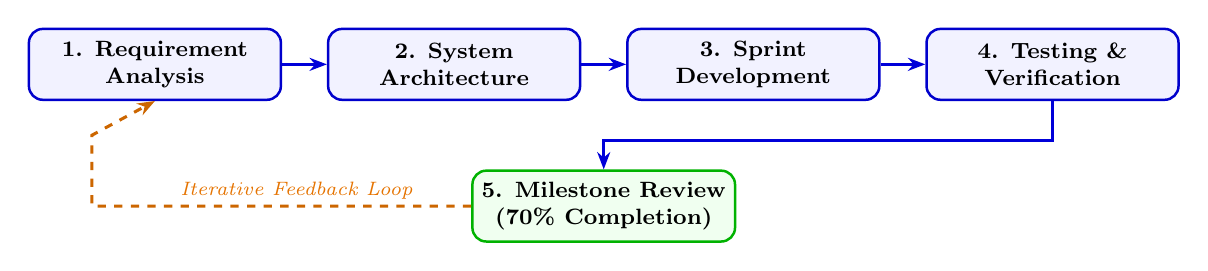
\begin{tikzpicture}[
    flowbox/.style={
        draw=blue!80!black,
        fill=blue!5!white,
        rounded corners=5pt,
        line width=0.9pt,
        minimum width=3.2cm,
        minimum height=0.9cm,
        font=\footnotesize\bfseries,
        align=center
    },
    arrow/.style={
        -{Stealth[length=2.2mm]},
        line width=1.1pt,
        draw=blue!85!black
    }
]
    \node[flowbox] (req) at (0, 0) {1. Requirement\\Analysis};
    \node[flowbox] (arch) at (3.8, 0) {2. System\\Architecture};
    \node[flowbox] (sprint) at (7.6, 0) {3. Sprint\\Development};
    \node[flowbox] (test) at (11.4, 0) {4. Testing \&\\Verification};
    \node[flowbox, draw=green!70!black, fill=green!6!white] (eval) at (5.7, -1.8) {5. Milestone Review\\(70\% Completion)};

    \draw[arrow] (req) -- (arch);
    \draw[arrow] (arch) -- (sprint);
    \draw[arrow] (sprint) -- (test);
    \draw[arrow] (test.south) -- ++(0,-0.5) -| (eval.north);
    \draw[arrow, dashed, draw=orange!80!black] (eval.west) -| (-0.8, -0.9) -- (req.south);
    \node[font=\scriptsize\itshape, text=orange!90!black] at (1.8, -1.6) {Iterative Feedback Loop};
\end{tikzpicture}
\caption{Iterative Engineering Methodology of AI Fitness Tracker}
\label{fig:methodology}
\end{figure}

\section{Exercise Catalog Structuring \& Data Processing}
The platform incorporates a verified catalog of 1,324 resistance movements categorized across 9 anatomical muscle regions (Chest, Back, Legs, Shoulders, Arms, Core, Glutes, Full Body, Cardio). Each movement record contains standardized metadata including movement mechanics (compound vs. isolation), required equipment, primary muscle groups, secondary stabilizers, and execution cues.

\section{Kinematic Pose Estimation \& Joint Angle Mathematics}
Exercise form evaluation and repetition counting are performed using skeletal keypoint trigonometry. Using 2D coordinates $(x, y)$ of three adjacent joints $A$, $B$ (vertex), and $C$, joint angle $\theta$ is derived using the vector dot product:
\begin{equation}
\cos(\theta) = \frac{\vec{BA} \cdot \vec{BC}}{|\vec{BA}| \, |\vec{BC}|}, \quad \theta = \arccos\left(\frac{(x_A - x_B)(x_C - x_B) + (y_A - y_B)(y_C - y_B)}{\sqrt{(x_A - x_B)^2 + (y_A - y_B)^2} \sqrt{(x_C - x_B)^2 + (y_C - y_B)^2}}\right) \times \frac{180^\circ}{\pi}
\end{equation}

A deterministic finite-state machine tracks transitions between eccentric (loading) and concentric (extension) phases:
\begin{table}[htbp]
\centering
\small
\renewcommand{\arraystretch}{1.25}
\begin{tabularx}{\textwidth}{|l|p{3.8cm}|p{3.4cm}|X|}
\hline
\textbf{Exercise} & \textbf{Tracked Keypoints} & \textbf{Concentric Phase ($\theta$)} & \textbf{Eccentric Phase ($\theta$)} \\
\hline
Push-Up & Shoulder, Elbow, Wrist & $\theta > 160^\circ$ (Lockout) & $\theta < 90^\circ$ (Chest to Floor) \\
\hline
Squat & Hip, Knee, Ankle & $\theta > 165^\circ$ (Full Extension) & $\theta < 95^\circ$ (Thigh Parallel) \\
\hline
Pull-Up & Shoulder, Elbow, Wrist & $\theta < 60^\circ$ (Chin Over Bar) & $\theta > 160^\circ$ (Dead Hang) \\
\hline
\end{tabularx}
\caption{Pose Estimation Biomechanical Repetition Thresholds}
\label{tab:kinematics_thresholds}
\end{table}

\section{Overall System Architecture}
The system architecture follows a decoupled three-tier design (Figure \ref{fig:system_arch}): Presentation Tier (React Native / Expo), Local Persistence Tier (SQLite write-ahead transaction queue), and Cloud Application Tier (Django REST Framework with PostgreSQL / Supabase).

\begin{figure}[htbp]
\centering
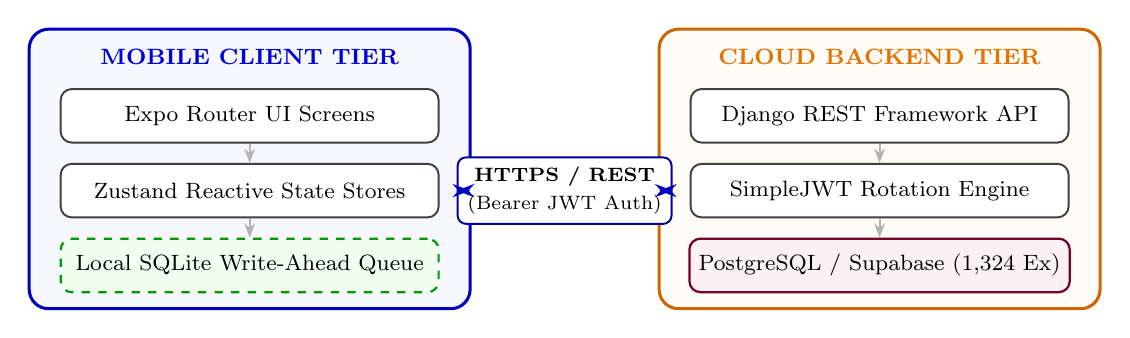
\begin{tikzpicture}[
    tierbox/.style={
        rounded corners=7pt,
        line width=1.1pt,
        inner sep=0pt
    },
    compnode/.style={
        draw=gray!50!black,
        fill=white,
        rounded corners=4pt,
        line width=0.7pt,
        minimum width=4.8cm,
        minimum height=0.68cm,
        font=\footnotesize,
        align=center
    },
    queuenode/.style={
        draw=green!60!black,
        fill=green!6!white,
        dashed,
        rounded corners=4pt,
        line width=0.8pt,
        minimum width=4.8cm,
        minimum height=0.68cm,
        font=\footnotesize,
        align=center
    },
    dbnode/.style={
        draw=purple!60!black,
        fill=purple!6!white,
        rounded corners=4pt,
        line width=0.8pt,
        minimum width=4.8cm,
        minimum height=0.68cm,
        font=\footnotesize,
        align=center
    }
]
    % --- MOBILE CLIENT TIER ---
    \draw[tierbox, draw=blue!75!black, fill=blue!3!white] (-6.8, -1.4) rectangle (-1.2, 2.15);
    \node[font=\bfseries\footnotesize, text=blue!85!black] at (-4.0, 1.8) {MOBILE CLIENT TIER};

    \node[compnode] (ui) at (-4.0, 1.05) {Expo Router UI Screens};
    \node[compnode] (state) at (-4.0, 0.1) {Zustand Reactive State Stores};
    \node[queuenode] (sqlite) at (-4.0, -0.85) {Local SQLite Write-Ahead Queue};

    \draw[-{Stealth[length=1.8mm]}, draw=gray!60, line width=0.7pt] (ui) -- (state);
    \draw[-{Stealth[length=1.8mm]}, draw=gray!60, line width=0.7pt] (state) -- (sqlite);

    % --- CLOUD BACKEND TIER ---
    \draw[tierbox, draw=orange!80!black, fill=orange!3!white] (1.2, -1.4) rectangle (6.8, 2.15);
    \node[font=\bfseries\footnotesize, text=orange!90!black] at (4.0, 1.8) {CLOUD BACKEND TIER};

    \node[compnode] (drf) at (4.0, 1.05) {Django REST Framework API};
    \node[compnode] (jwt) at (4.0, 0.1) {SimpleJWT Rotation Engine};
    \node[dbnode] (db) at (4.0, -0.85) {PostgreSQL / Supabase (1,324 Ex)};

    \draw[-{Stealth[length=1.8mm]}, draw=gray!60, line width=0.7pt] (drf) -- (jwt);
    \draw[-{Stealth[length=1.8mm]}, draw=gray!60, line width=0.7pt] (jwt) -- (db);

    % --- COMMUNICATION LINK (CENTER) ---
    \node[
        draw=blue!60!black,
        fill=white,
        rounded corners=3pt,
        line width=0.7pt,
        font=\scriptsize,
        align=center,
        inner sep=3.5pt
    ] (proto) at (0, 0.1) {
        \textbf{HTTPS / REST}\\[2pt]
        \scriptsize (Bearer JWT Auth)
    };

    \draw[{Stealth[length=2.2mm]}-{Stealth[length=2.2mm]}, line width=1.2pt, draw=blue!75!black] (-1.2, 0.1) -- (proto.west);
    \draw[{Stealth[length=2.2mm]}-{Stealth[length=2.2mm]}, line width=1.2pt, draw=blue!75!black] (proto.east) -- (1.2, 0.1);
\end{tikzpicture}
\caption{Overall System Architecture of AI Fitness Tracker}
\label{fig:system_arch}
\end{figure}

\section{Use Case Model}
The interaction boundaries between the athlete trainee, local offline persistence, and cloud services are represented in Figure \ref{fig:use_case}.

\begin{figure}[htbp]
\centering
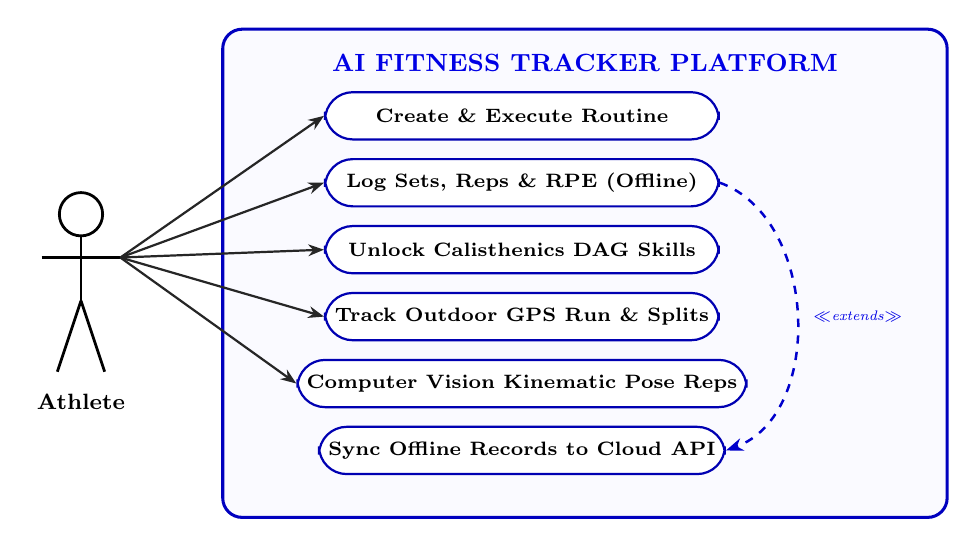
\begin{tikzpicture}[
    ucnode/.style={
        draw=blue!70!black,
        fill=white,
        rounded corners=10pt,
        line width=0.8pt,
        minimum width=5.0cm,
        minimum height=0.6cm,
        font=\scriptsize\bfseries,
        align=center
    }
]
    % System boundary
    \draw[rounded corners=7pt, line width=1.1pt, draw=blue!75!black, fill=blue!2!white] (0, -0.45) rectangle (9.2, 5.75);
    \node[anchor=north, font=\small\bfseries, text=blue!90!black] at (4.6, 5.55) {AI FITNESS TRACKER PLATFORM};

    % Athlete Actor
    \coordinate (actorcenter) at (-1.8, 2.7);
    \node[draw=black, line width=1pt, circle, fill=white, minimum size=0.55cm] (head) at (-1.8, 3.4) {};
    \draw[line width=1pt] (head.south) -- (-1.8, 2.3) coordinate (pelvis);
    \draw[line width=1pt] (-2.3, 2.85) -- (-1.3, 2.85) coordinate (hands);
    \draw[line width=1pt] (pelvis) -- (-2.1, 1.4);
    \draw[line width=1pt] (pelvis) -- (-1.5, 1.4);
    \node[below=3pt, font=\footnotesize\bfseries] at (-1.8, 1.35) {Athlete};

    % Use Cases
    \node[ucnode] (uc1) at (3.8, 4.65) {Create \& Execute Routine};
    \node[ucnode] (uc2) at (3.8, 3.8) {Log Sets, Reps \& RPE (Offline)};
    \node[ucnode] (uc3) at (3.8, 2.95) {Unlock Calisthenics DAG Skills};
    \node[ucnode] (uc4) at (3.8, 2.1) {Track Outdoor GPS Run \& Splits};
    \node[ucnode] (uc5) at (3.8, 1.25) {Computer Vision Kinematic Pose Reps};
    \node[ucnode] (uc6) at (3.8, 0.4) {Sync Offline Records to Cloud API};

    % Associations
    \draw[-{Stealth[length=2mm]}, line width=0.8pt, draw=black!85] (hands) -- (uc1.west);
    \draw[-{Stealth[length=2mm]}, line width=0.8pt, draw=black!85] (hands) -- (uc2.west);
    \draw[-{Stealth[length=2mm]}, line width=0.8pt, draw=black!85] (hands) -- (uc3.west);
    \draw[-{Stealth[length=2mm]}, line width=0.8pt, draw=black!85] (hands) -- (uc4.west);
    \draw[-{Stealth[length=2mm]}, line width=0.8pt, draw=black!85] (hands) -- (uc5.west);

    % Extends relationship
    \draw[dashed, -{Stealth[length=2.2mm]}, line width=0.9pt, draw=blue!80!black] 
        (uc2.east) to[out=-20, in=20] 
        node[midway, right=2pt, font=\tiny\itshape, text=blue!90!black] {$\ll$extends$\gg$} 
        (uc6.east);
\end{tikzpicture}
\caption{Use Case Diagram of AI Fitness Tracker Platform}
\label{fig:use_case}
\end{figure}

\section{Sequence Model: Offline Persistence \& Cloud Synchronization}
Figure \ref{fig:seq_diagram} details the sequential execution flow during active workout set logging and subsequent cloud synchronization.

\begin{figure}[htbp]
\centering
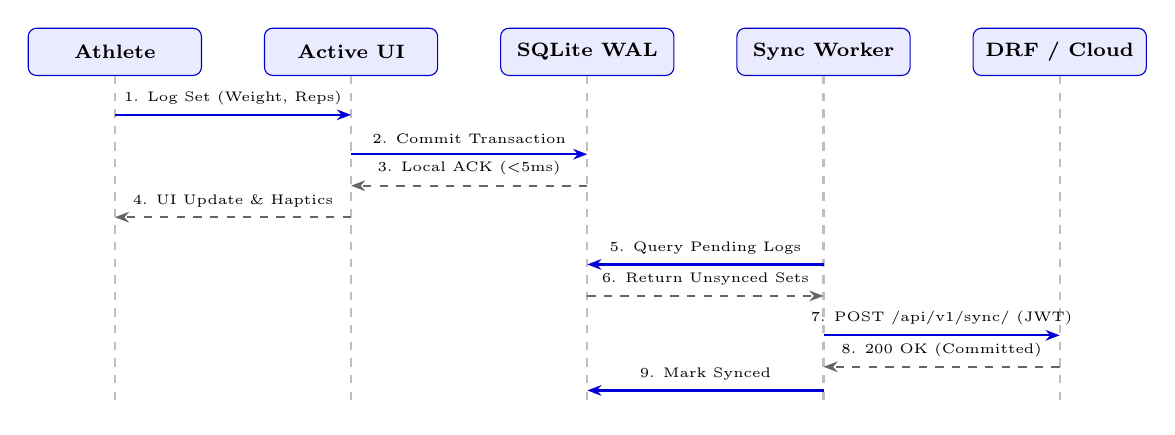
\begin{tikzpicture}[
    lifeline/.style={draw=gray!50, line width=0.8pt, dashed},
    box/.style={draw=blue!80!black, fill=blue!8!white, rounded corners=3pt, font=\scriptsize\bfseries, align=center, minimum width=2.2cm, minimum height=0.6cm},
    msg/.style={-{Stealth[length=1.8mm]}, line width=0.8pt, draw=blue!85!black, font=\tiny},
    reply/.style={-{Stealth[length=1.8mm]}, line width=0.8pt, dashed, draw=gray!80!black, font=\tiny}
]
    % Participants
    \node[box] (ath) at (0, 0) {Athlete};
    \node[box] (ui) at (3.0, 0) {Active UI};
    \node[box] (sql) at (6.0, 0) {SQLite WAL};
    \node[box] (sync) at (9.0, 0) {Sync Worker};
    \node[box] (api) at (12.0, 0) {DRF / Cloud};

    % Lifelines
    \draw[lifeline] (ath) -- (0, -4.5);
    \draw[lifeline] (ui) -- (3.0, -4.5);
    \draw[lifeline] (sql) -- (6.0, -4.5);
    \draw[lifeline] (sync) -- (9.0, -4.5);
    \draw[lifeline] (api) -- (12.0, -4.5);

    % Messages
    \draw[msg] (0, -0.8) -- node[above]{1. Log Set (Weight, Reps)} (3.0, -0.8);
    \draw[msg] (3.0, -1.3) -- node[above]{2. Commit Transaction} (6.0, -1.3);
    \draw[reply] (6.0, -1.7) -- node[above]{3. Local ACK (<5ms)} (3.0, -1.7);
    \draw[reply] (3.0, -2.1) -- node[above]{4. UI Update \& Haptics} (0, -2.1);

    \draw[msg] (9.0, -2.7) -- node[above]{5. Query Pending Logs} (6.0, -2.7);
    \draw[reply] (6.0, -3.1) -- node[above]{6. Return Unsynced Sets} (9.0, -3.1);
    \draw[msg] (9.0, -3.6) -- node[above]{7. POST /api/v1/sync/ (JWT)} (12.0, -3.6);
    \draw[reply] (12.0, -4.0) -- node[above]{8. 200 OK (Committed)} (9.0, -4.0);
    \draw[msg] (9.0, -4.3) -- node[above]{9. Mark Synced} (6.0, -4.3);
\end{tikzpicture}
\caption{Sequence Diagram for Offline Workout Logging \& Cloud Synchronization}
\label{fig:seq_diagram}
\end{figure}

\section{Database Schema \& Relational Models}
The database architecture employs PostgreSQL on the cloud backend and a mirror schema in SQLite on the mobile client (Table \ref{tab:db_schema}).

\begin{table}[htbp]
\centering
\small
\renewcommand{\arraystretch}{1.25}
\begin{tabularx}{\textwidth}{|l|p{4.5cm}|X|}
\hline
\textbf{Table Name} & \textbf{Key Attributes} & \textbf{Functional Purpose} \\
\hline
\texttt{User} & \texttt{id (UUID), email, password, createdAt} & Primary athlete authentication. \\
\hline
\texttt{UserProfile} & \texttt{userId, displayName, units, experience} & Athlete profile configurations. \\
\hline
\texttt{Exercise} & \texttt{id, name, type, muscleGroup, equipment} & 1,324 exercise movement catalog. \\
\hline
\texttt{Routine} & \texttt{id, userId, name, category, exercises} & Reusable workout templates. \\
\hline
\texttt{WorkoutSession} & \texttt{id, userId, startTime, endTime, volume} & Audit record of completed workouts. \\
\hline
\texttt{WorkoutSet} & \texttt{id, sessionId, exerciseId, weightKg, reps, rpe} & Set-by-set performance metrics. \\
\hline
\texttt{PersonalRecord} & \texttt{id, userId, exerciseId, type, value} & Milestone PR records. \\
\hline
\texttt{RunSession} & \texttt{id, userId, distanceMeters, avgPace, polyline} & Outdoor GPS running sessions. \\
\hline
\end{tabularx}
\caption{Relational Database Schema \& Data Models}
\label{tab:db_schema}
\end{table}

\chapter{IMPLEMENTATION DETAILS}

\section{Backend Implementation}
The backend is structured as a modular Django REST Framework (DRF) application organized across domain-specific apps (\texttt{users}, \texttt{exercises}, \texttt{workouts}, \texttt{routines}, and \texttt{runs}). The authentication subsystem utilizes \textbf{SimpleJWT} to issue short-lived access tokens (15-minute expiration) and rotating refresh tokens (7-day validity). All database operations utilize PostgreSQL hosted on Supabase, with complete OpenAPI 3.0 schema generation for contract testing.

\section{Mobile Frontend Development}
The client application is built with \textbf{React Native} using the \textbf{Expo SDK 52} managed workflow. Application routing is handled declaratively using \textbf{Expo Router} with file-based hierarchical navigation. Reactive state management is implemented via \textbf{Zustand}, utilizing custom storage adapters that bridge in-memory state with \textbf{Expo SQLite} and \textbf{AsyncStorage}.

\section{Core Subsystem Engineering}

\subsection{Active Workout Logging \& Automated PR Detection}
The active workout engine in \texttt{activeWorkoutStore.ts} pre-fills weight and repetition targets from prior logs. Upon set completion, the system calculates estimated 1RM using the Brzycki formula:
\begin{equation}
1\text{RM} = \frac{w}{1.0278 - 0.0278 \cdot r}
\end{equation}
Personal Records are evaluated across three discrete metrics: Max Weight, Max Volume, and Max Reps. Audio-haptic rest timers automatically trigger upon set completion.

\subsection{Calisthenics Directed Acyclic Graph (DAG) Progression Trees}
Bodyweight movements are structured as nodes within five discipline Directed Acyclic Graphs (Push, Pull, Legs, Core, and Handstand). Each node defines prerequisite mastery nodes and quantitative unlock criteria (e.g., executing 3 sets of 12 clean dips before unlocking Muscle-Up progression).

\subsection{Outdoor GPS Run Tracking \& Spatial Smoothing}
Location tracking operates via an active Android foreground service (\texttt{expo-task-manager}). Geospatial distance accumulates using the Haversine formula:
\begin{equation}
d = 2R \arcsin\left(\sqrt{\sin^2\left(\frac{\Delta \text{lat}}{2}\right) + \cos(\text{lat}_1)\cos(\text{lat}_2)\sin^2\left(\frac{\Delta \text{lon}}{2}\right)}\right)
\end{equation}
Coordinates with horizontal accuracy error greater than 15 meters are discarded. Rolling 30-second moving windows smooth momentary GPS speed spikes, and audio pace splits announce progress per completed kilometer.

\subsection{MediaPipe BlazePose Kinematics HUD}
The computer vision subsystem processes camera frames on-device, extracting 33 keypoints to derive real-time joint flexion angles. The finite-state machine validates rep completion and form violations (such as asymmetric elbow flaring or incomplete squat depth) without transmitting video data off the device.

\clearpage

\section{User Interface Implementation}
The client application implements a high-contrast OLED dark design system optimized for gym environments and low-light athletic settings. Figures \ref{fig:login_screen} through \ref{fig:settings_profile} present the operational interfaces captured from the live application runtime arranged in serial order across the user journey---from initial authentication and onboarding, to daily dashboard metrics and routine planning, active resistance workout logging and edge computer vision form analysis, calisthenics skill mastery and outdoor GPS running telemetry, to community social interaction, scientific knowledge insights, squad challenges, and athlete configuration settings.

\subsection{Athlete Authentication and Account Registration}
Figure \ref{fig:login_screen} illustrates the athlete sign-in portal featuring secure JWT credential authentication, offline demo bypass, and server connectivity diagnostics. Figure \ref{fig:signup_screen} displays the registration screen facilitating new athlete onboarding with credential validation and profile initialization.

\begin{figure}[htbp]
\centering
\begin{minipage}[t]{0.48\textwidth}
    \centering
    \IfFileExists{screenshots/login_screen.png}{
        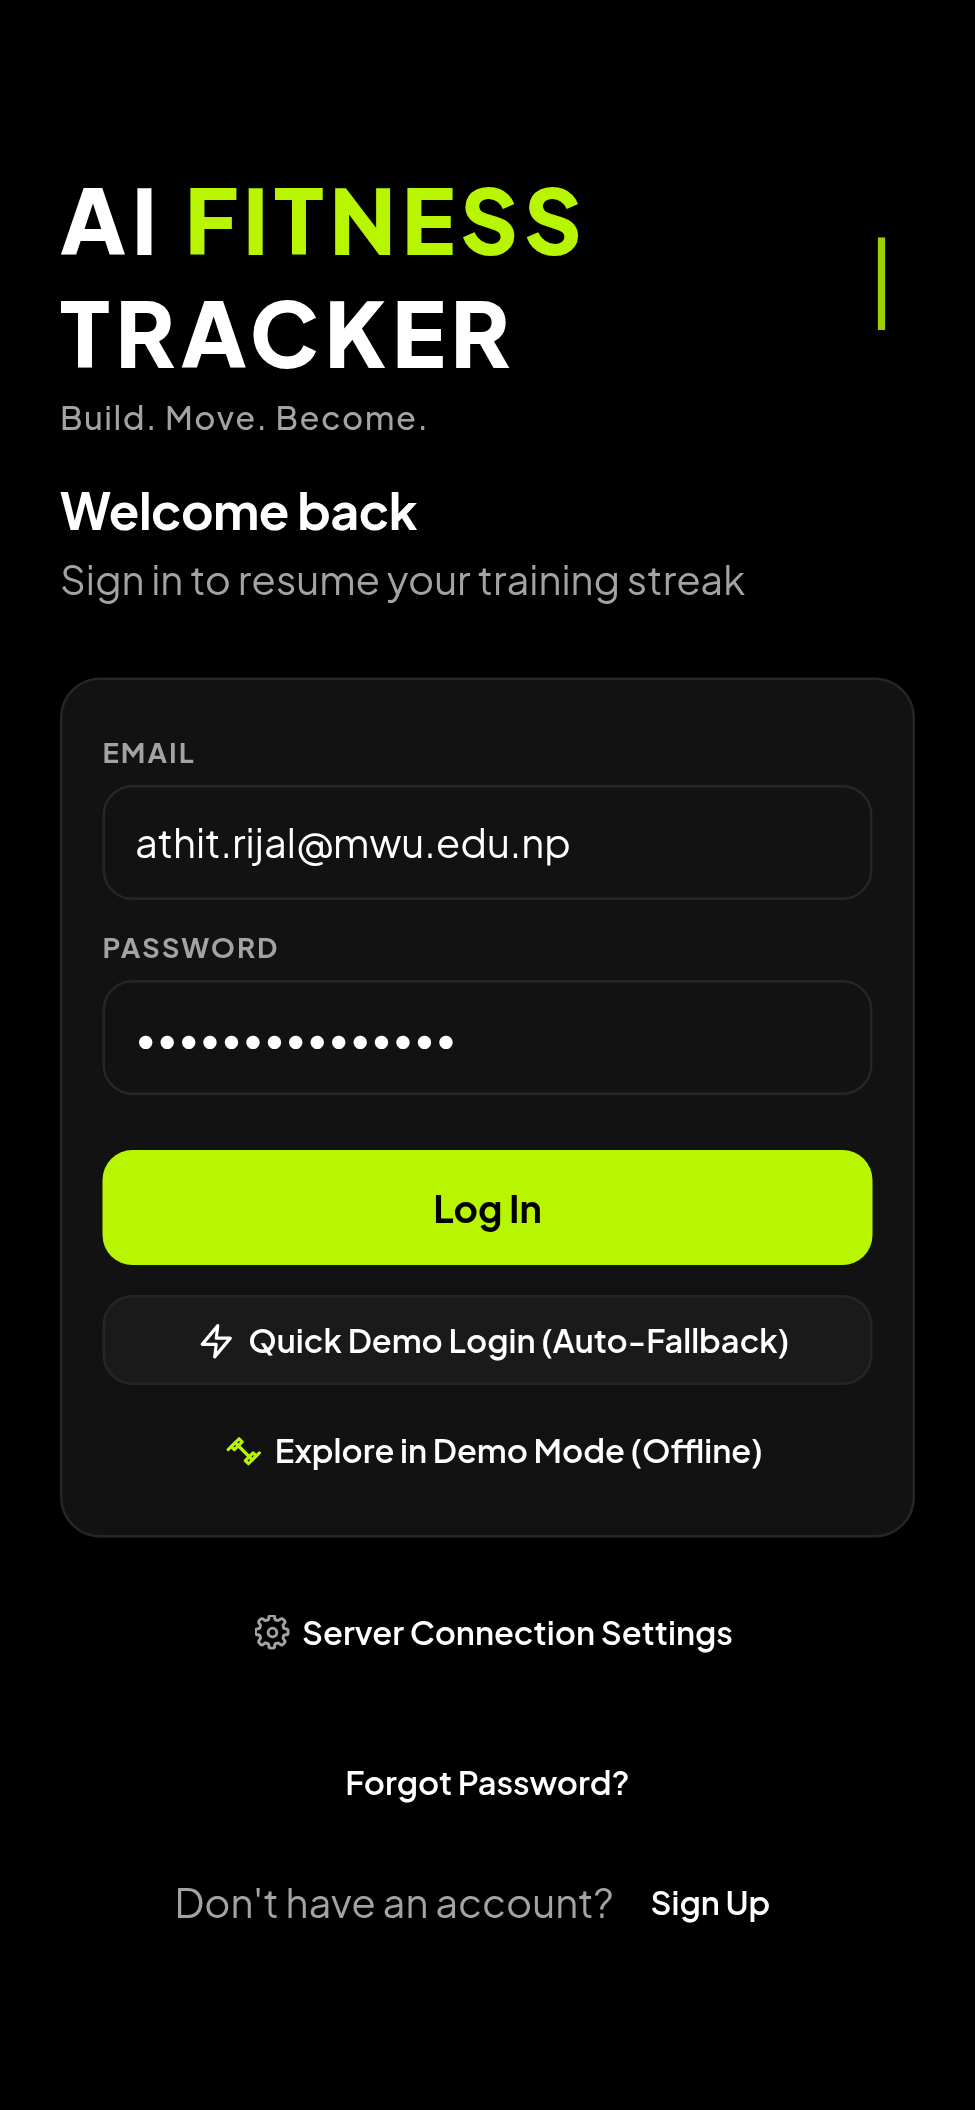
\includegraphics[height=9.8cm,keepaspectratio]{screenshots/login_screen.png}
    }{
        \fbox{\parbox[c][5.5cm][c]{0.9\textwidth}{\centering \textbf{[ Athlete Login ]}}}
    }
    \caption{Athlete Login \& Credential Authentication Interface}
    \label{fig:login_screen}
\end{minipage}
\hfill
\begin{minipage}[t]{0.48\textwidth}
    \centering
    \IfFileExists{screenshots/signup_screen.png}{
        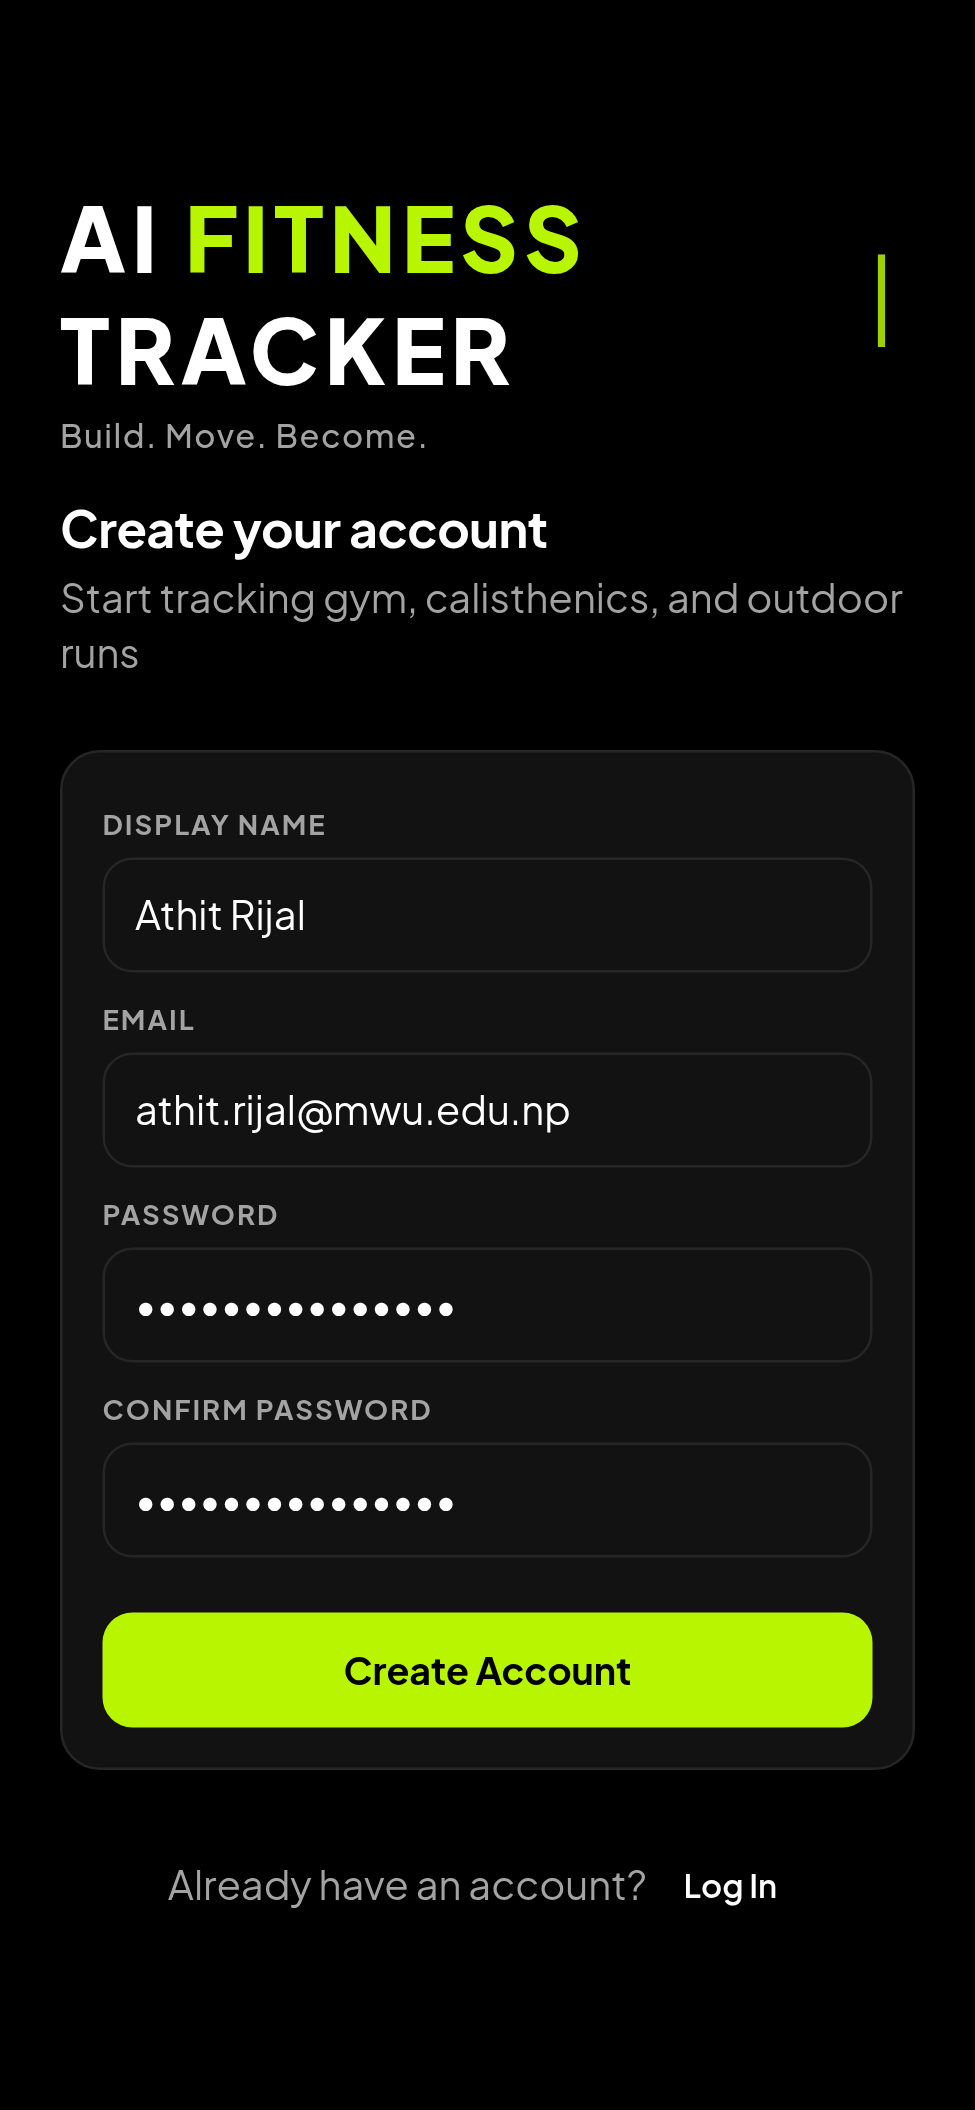
\includegraphics[height=9.8cm,keepaspectratio]{screenshots/signup_screen.png}
    }{
        \fbox{\parbox[c][5.5cm][c]{0.9\textwidth}{\centering \textbf{[ Athlete Sign Up ]}}}
    }
    \caption{New Athlete Registration \& Account Creation Interface}
    \label{fig:signup_screen}
\end{minipage}
\end{figure}

\clearpage

\subsection{Activity Dashboard and Custom Routine Planning}
Figure \ref{fig:dashboard} showcases the Today Dashboard summarizing training streaks, total tonnage volume, and an annual consistency heatmap. Figure \ref{fig:routine_builder} illustrates the Custom Routine Builder featuring interactive superset grouping and automated muscle group coverage analysis.

\begin{figure}[htbp]
\centering
\begin{minipage}[t]{0.48\textwidth}
    \centering
    \IfFileExists{screenshots/dashboard_screen.png}{
        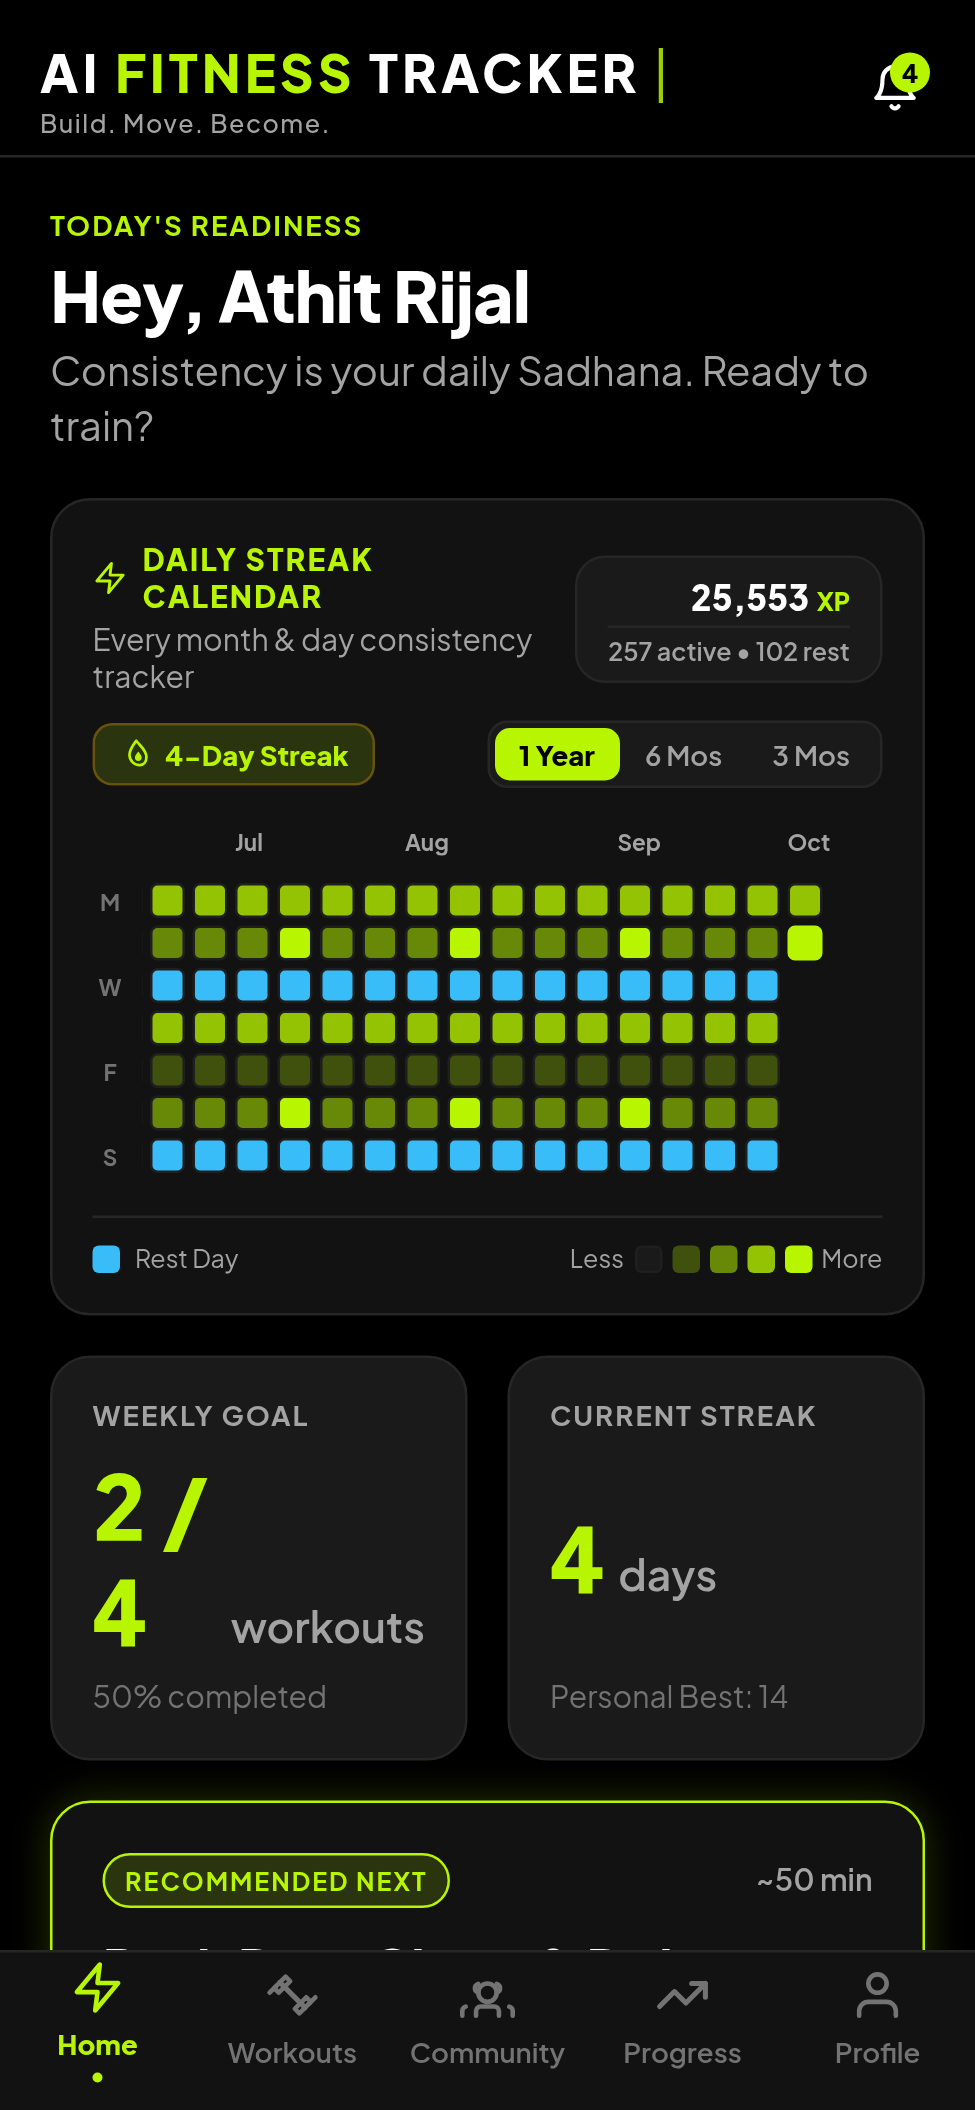
\includegraphics[height=11.0cm,keepaspectratio]{screenshots/dashboard_screen.png}
    }{
        \fbox{\parbox[c][5.5cm][c]{0.9\textwidth}{\centering \textbf{[ Athlete Dashboard ]}}}
    }
    \caption{Today Dashboard \& Annual Consistency Heatmap}
    \label{fig:dashboard}
\end{minipage}
\hfill
\begin{minipage}[t]{0.48\textwidth}
    \centering
    \IfFileExists{screenshots/routine_builder_screen.png}{
        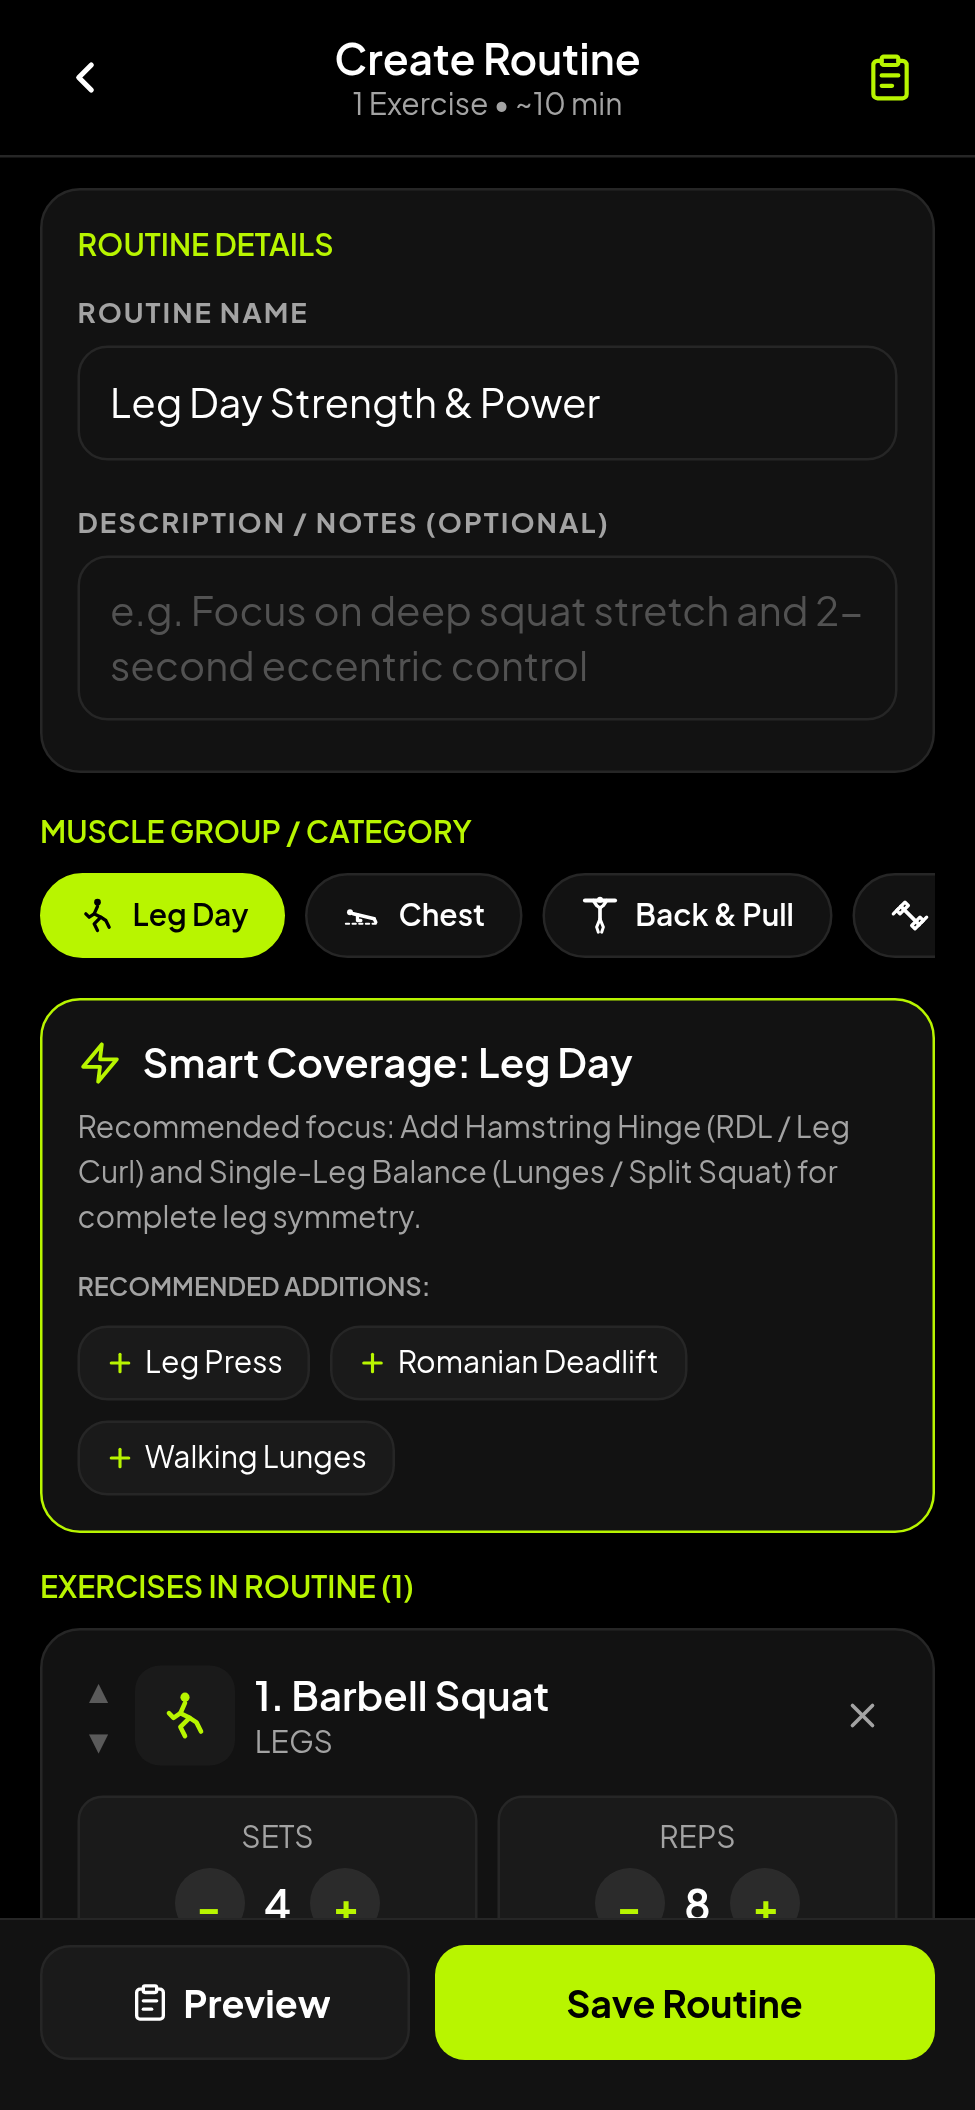
\includegraphics[height=11.0cm,keepaspectratio]{screenshots/routine_builder_screen.png}
    }{
        \fbox{\parbox[c][5.5cm][c]{0.9\textwidth}{\centering \textbf{[ Routine Builder ]}}}
    }
    \caption{Custom Routine Builder \& Muscle Coverage Analysis}
    \label{fig:routine_builder}
\end{minipage}
\end{figure}

\clearpage

\subsection{Active Workout Logging and Real-Time Form Kinematics}
Figure \ref{fig:workout_logger} illustrates the active workout logger with live set tracking, RPE ratings, muscle targeting badges, and rest timers. Figure \ref{fig:vision_tracker} exhibits the on-device Computer Vision Pose Tracker HUD performing real-time MediaPipe skeletal joint angle analysis and rep counting.

\begin{figure}[htbp]
\centering
\begin{minipage}[t]{0.48\textwidth}
    \centering
    \IfFileExists{screenshots/workout_screen.png}{
        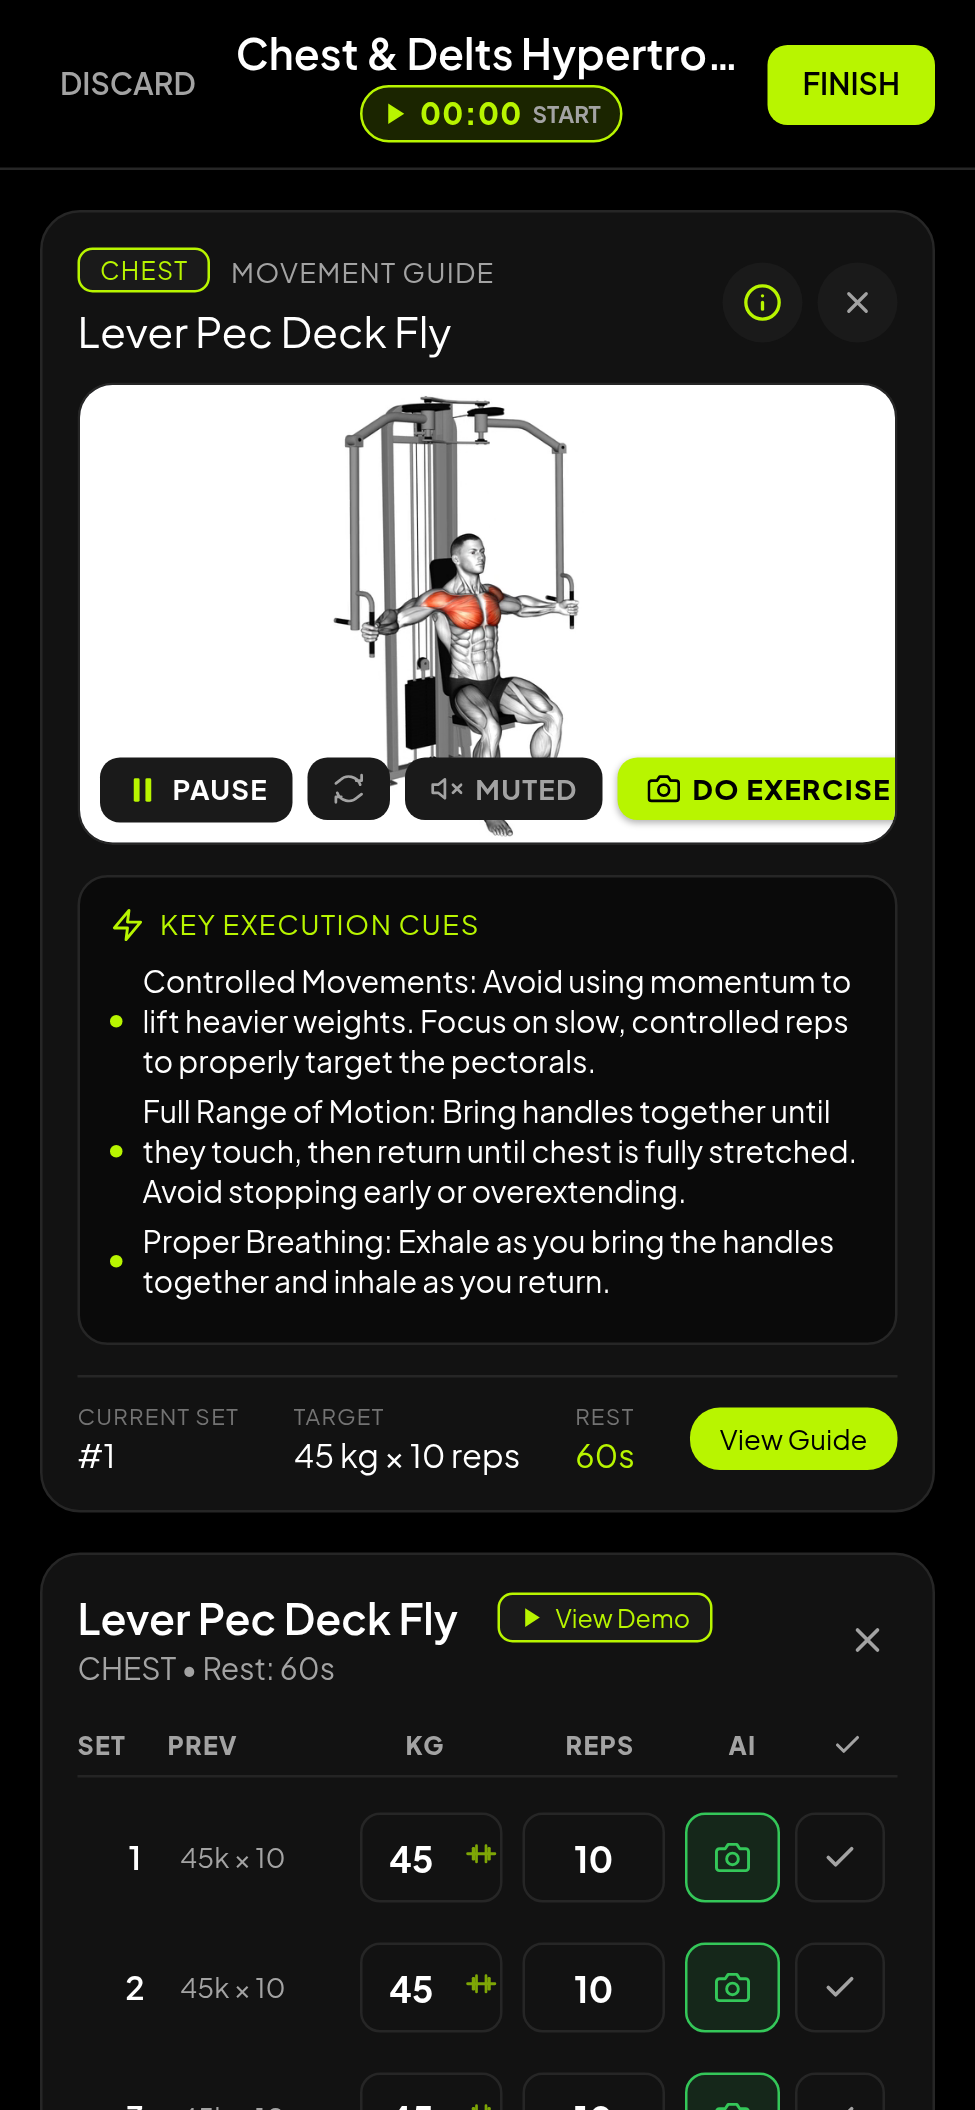
\includegraphics[height=11.0cm,keepaspectratio]{screenshots/workout_screen.png}
    }{
        \fbox{\parbox[c][5.5cm][c]{0.9\textwidth}{\centering \textbf{[ Active Workout Logger ]}}}
    }
    \caption{Active Workout Logger \& Live Set Tracking Interface}
    \label{fig:workout_logger}
\end{minipage}
\hfill
\begin{minipage}[t]{0.48\textwidth}
    \centering
    \IfFileExists{screenshots/vision_tracker_screen.png}{
        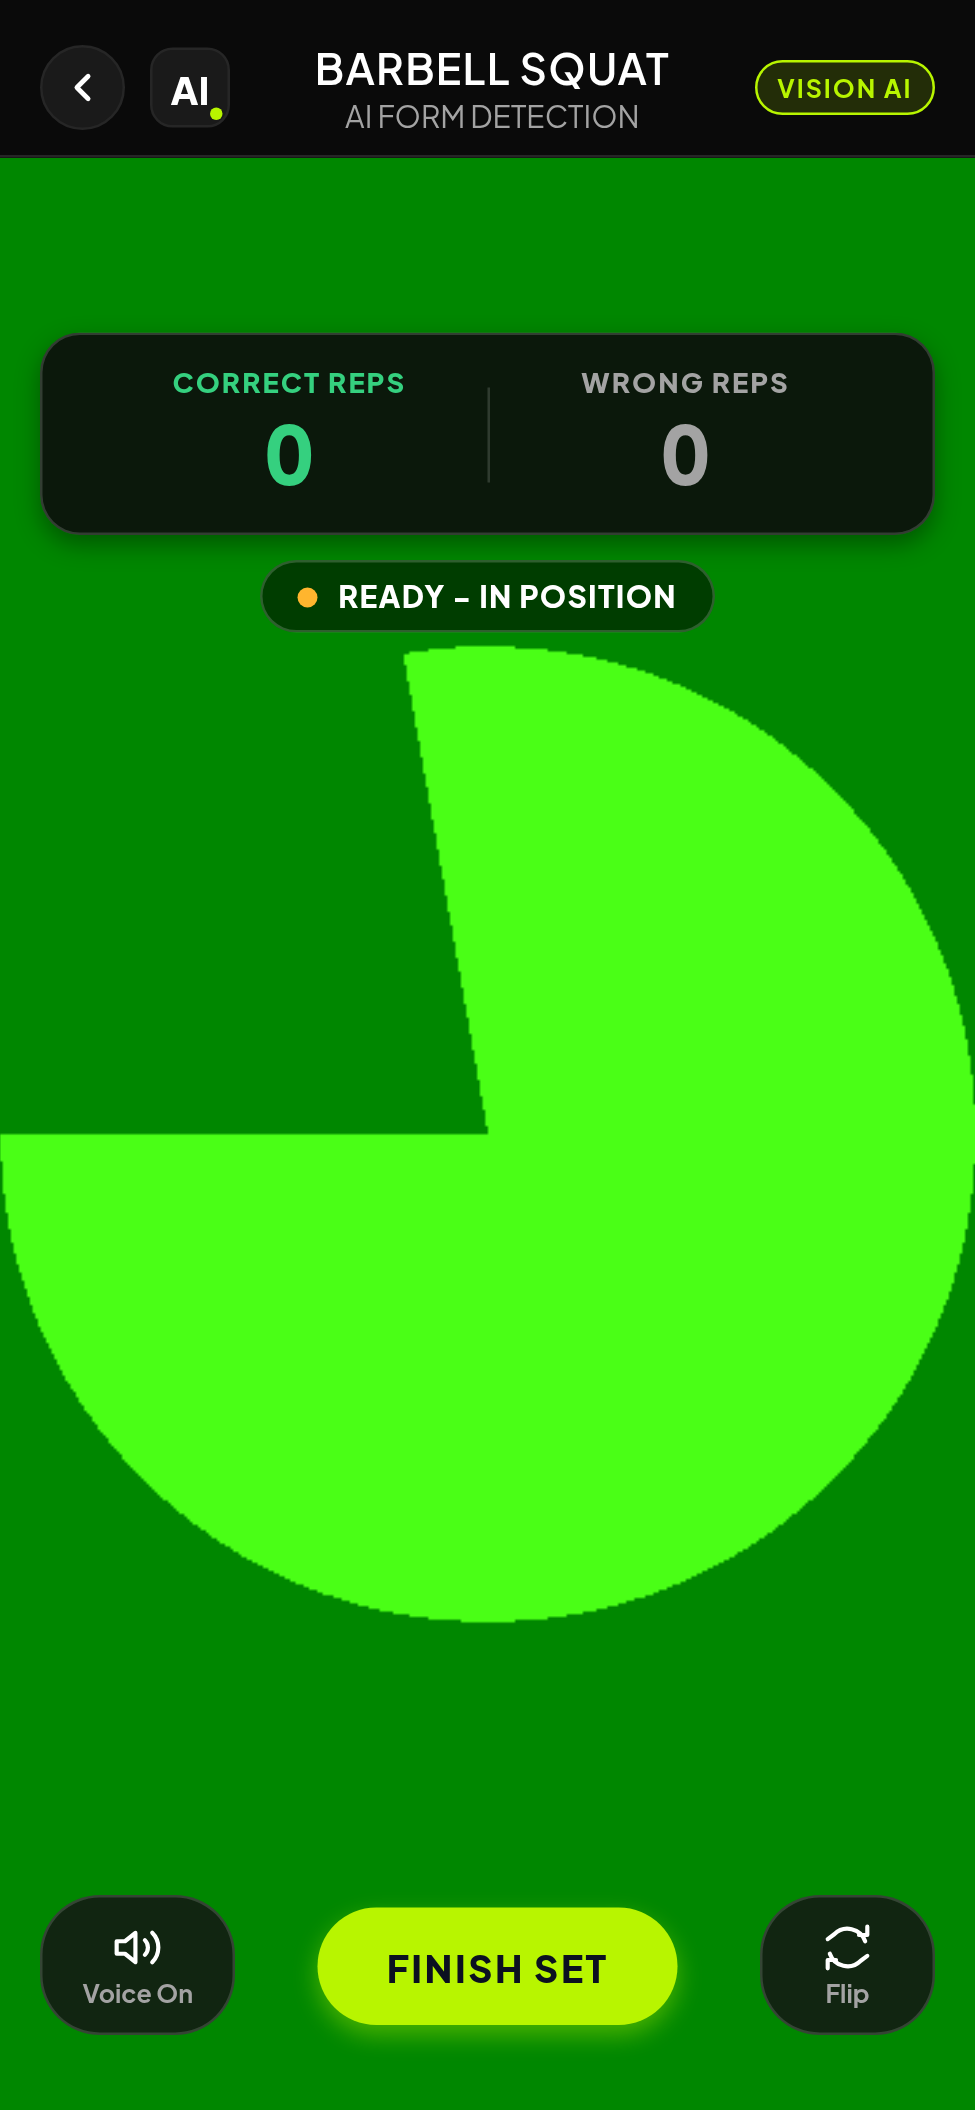
\includegraphics[height=11.0cm,keepaspectratio]{screenshots/vision_tracker_screen.png}
    }{
        \fbox{\parbox[c][5.5cm][c]{0.9\textwidth}{\centering \textbf{[ Vision Pose Tracker ]}}}
    }
    \caption{Computer Vision Kinematic Pose Rep Tracker HUD}
    \label{fig:vision_tracker}
\end{minipage}
\end{figure}

\clearpage

\subsection{Calisthenics Skill Tree and Outdoor GPS Running}
Figure \ref{fig:skilltree} demonstrates the Calisthenics Skill Tree displaying Warrior Rank ascension and prerequisite unlock nodes across five movement branches. Figure \ref{fig:gps_run} presents the outdoor running telemetry interface featuring satellite route mapping, real-time pace, and distance accumulation.

\begin{figure}[htbp]
\centering
\begin{minipage}[t]{0.48\textwidth}
    \centering
    \IfFileExists{screenshots/skilltree_screen.png}{
        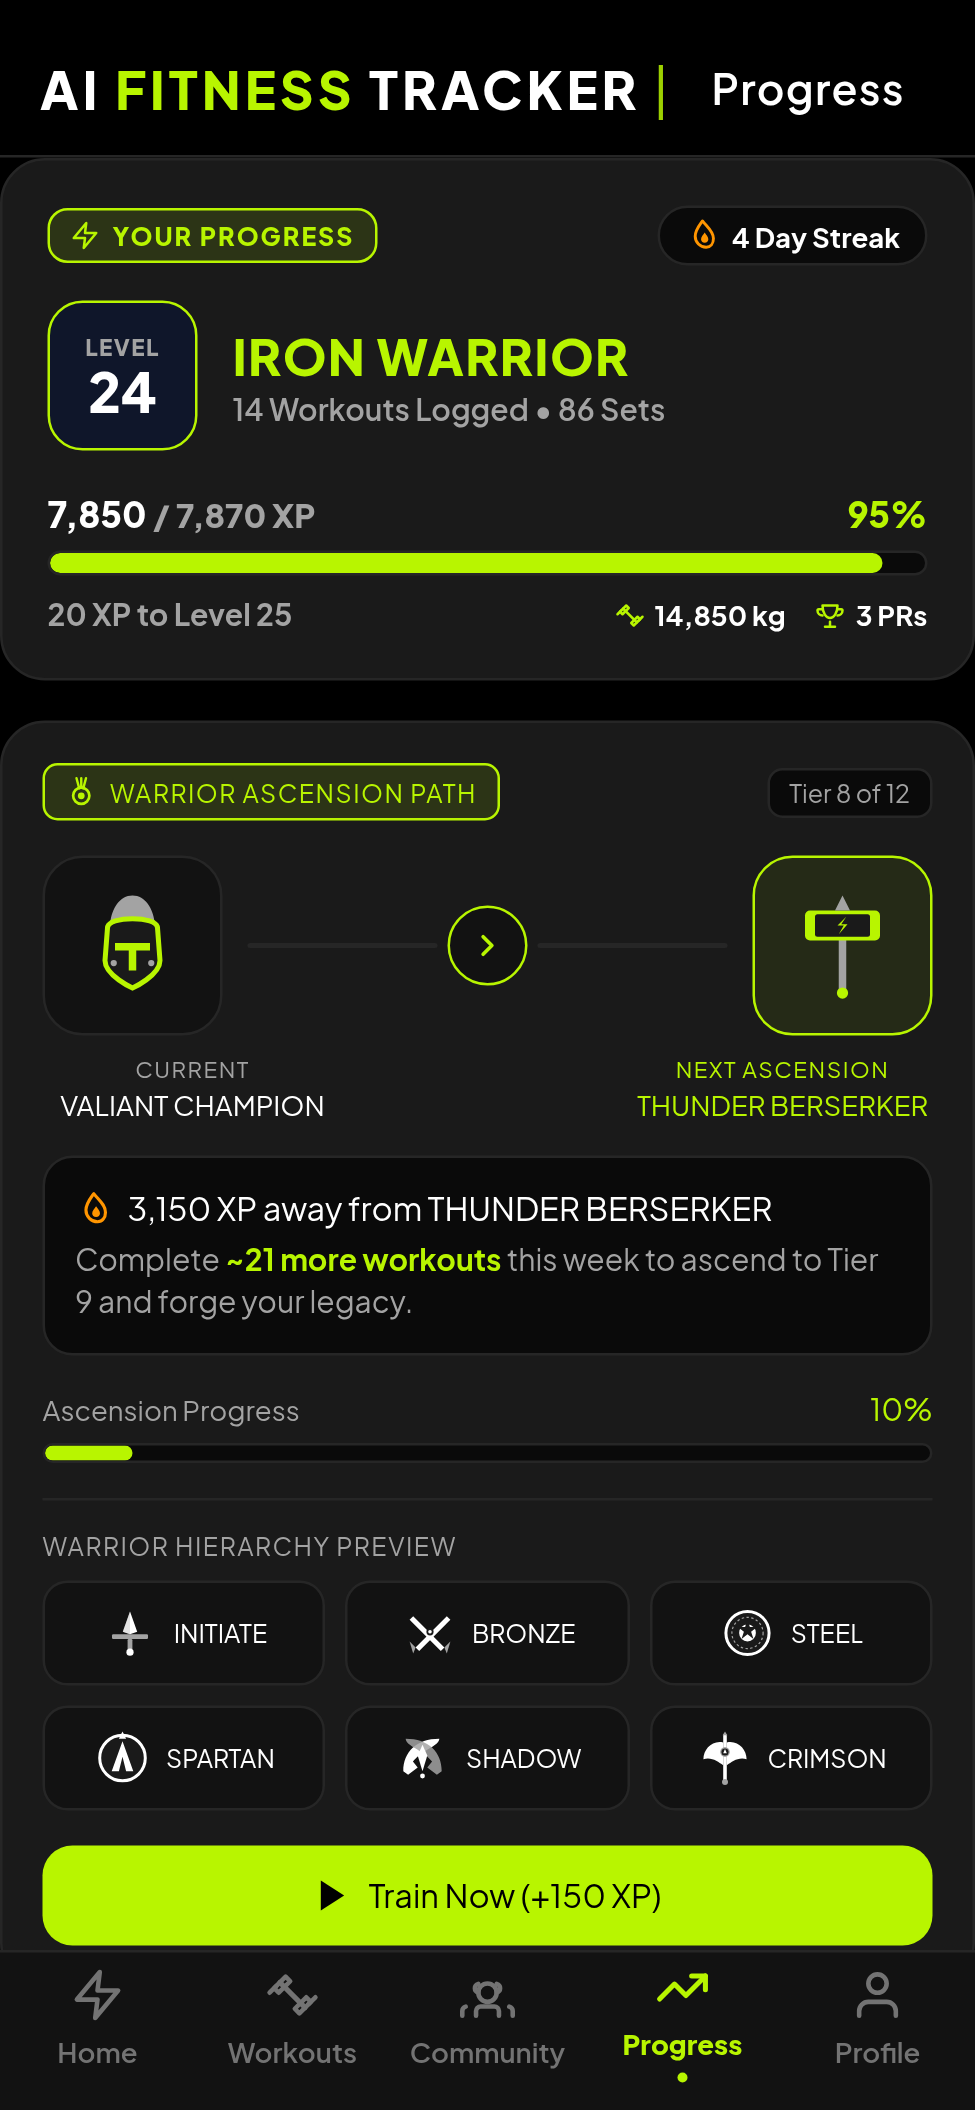
\includegraphics[height=11.0cm,keepaspectratio]{screenshots/skilltree_screen.png}
    }{
        \fbox{\parbox[c][5.5cm][c]{0.9\textwidth}{\centering \textbf{[ Skill Tree \& Progression ]}}}
    }
    \caption{Warrior Rank Ascension \& Skill Progression Interface}
    \label{fig:skilltree}
\end{minipage}
\hfill
\begin{minipage}[t]{0.48\textwidth}
    \centering
    \IfFileExists{screenshots/gps_run_screen.png}{
        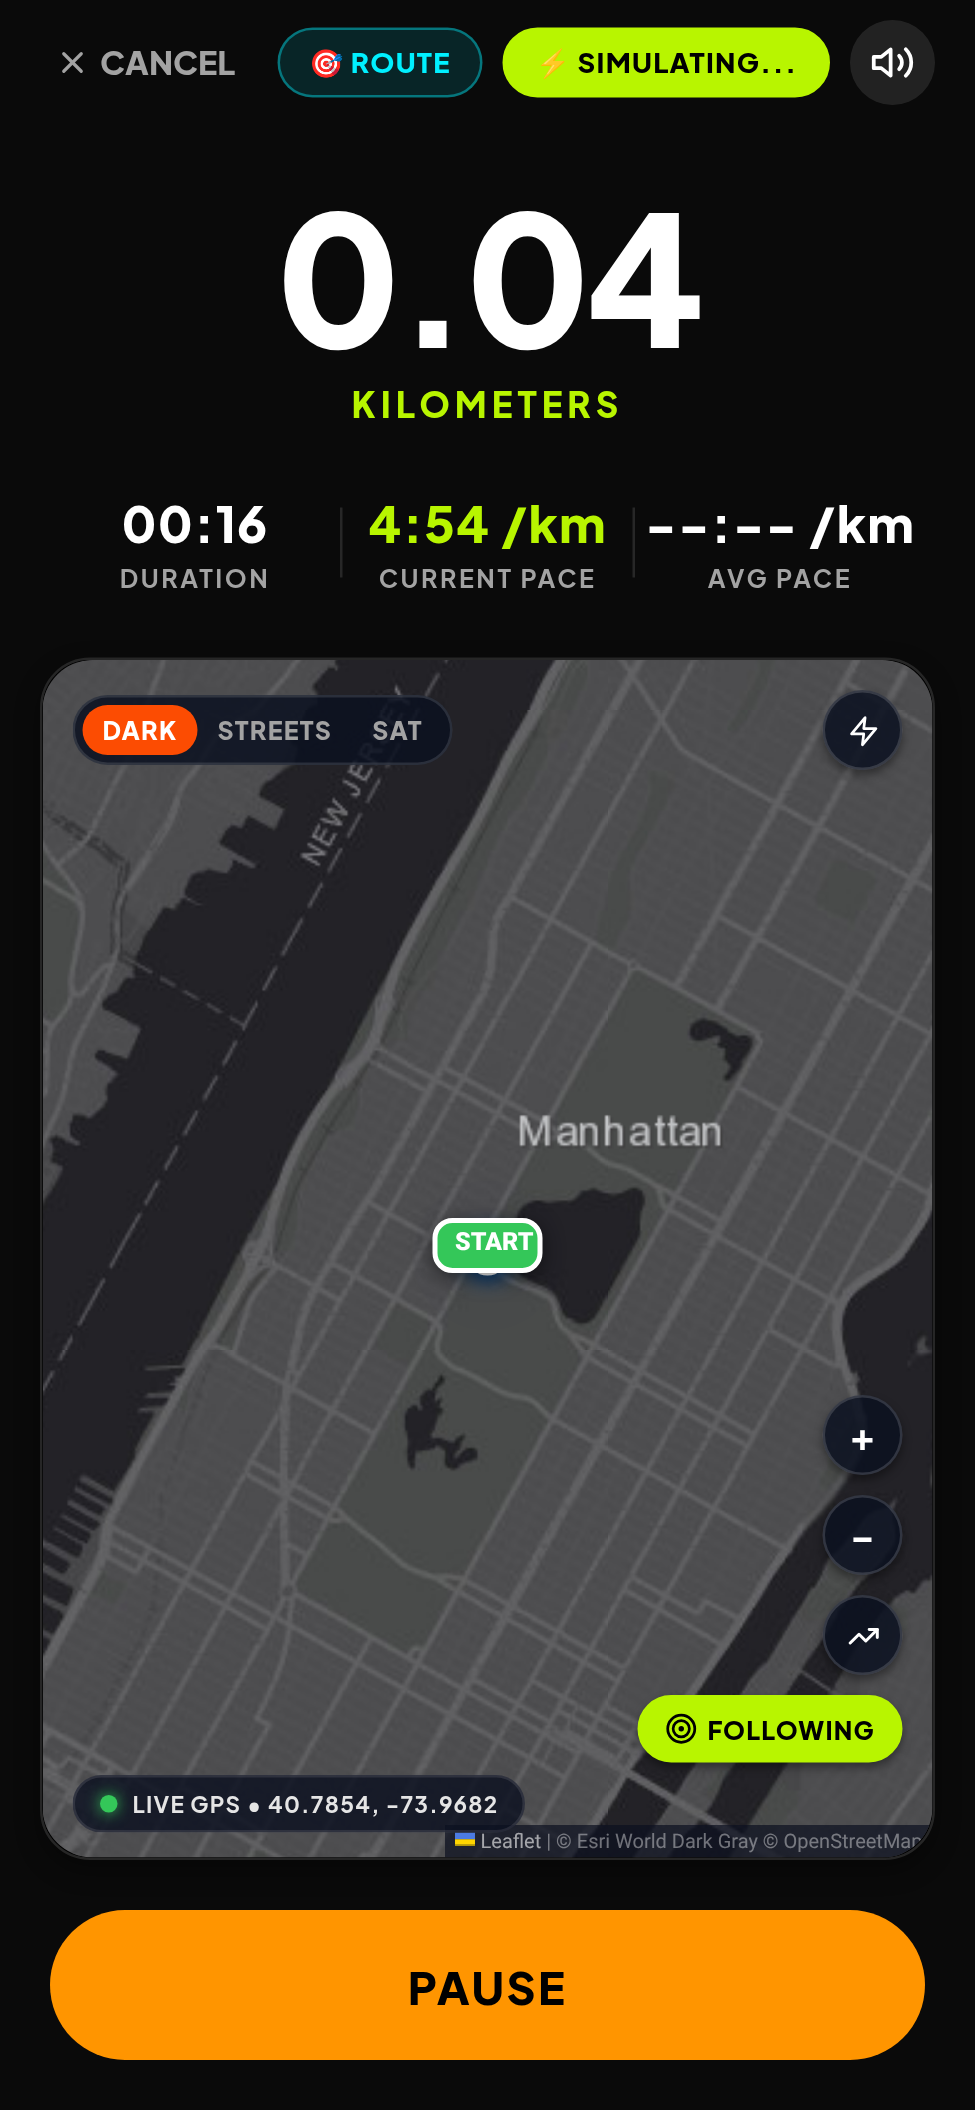
\includegraphics[height=11.0cm,keepaspectratio]{screenshots/gps_run_screen.png}
    }{
        \fbox{\parbox[c][5.5cm][c]{0.9\textwidth}{\centering \textbf{[ GPS Run Tracker ]}}}
    }
    \caption{Outdoor GPS Run Tracking \& Real-Time Route Interface}
    \label{fig:gps_run}
\end{minipage}
\end{figure}

\clearpage

\subsection{Community Social Feed and Scientific Knowledge Insights}
Figure \ref{fig:community_feed} illustrates the Squad Social Feed for peer workout sharing, athletic encouragement, and community kudos. Figure \ref{fig:community_insights} showcases the Evidence-Based Science tab curating peer-reviewed training methodologies and biomechanics literature.

\begin{figure}[htbp]
\centering
\begin{minipage}[t]{0.48\textwidth}
    \centering
    \IfFileExists{screenshots/community_feed_screen.png}{
        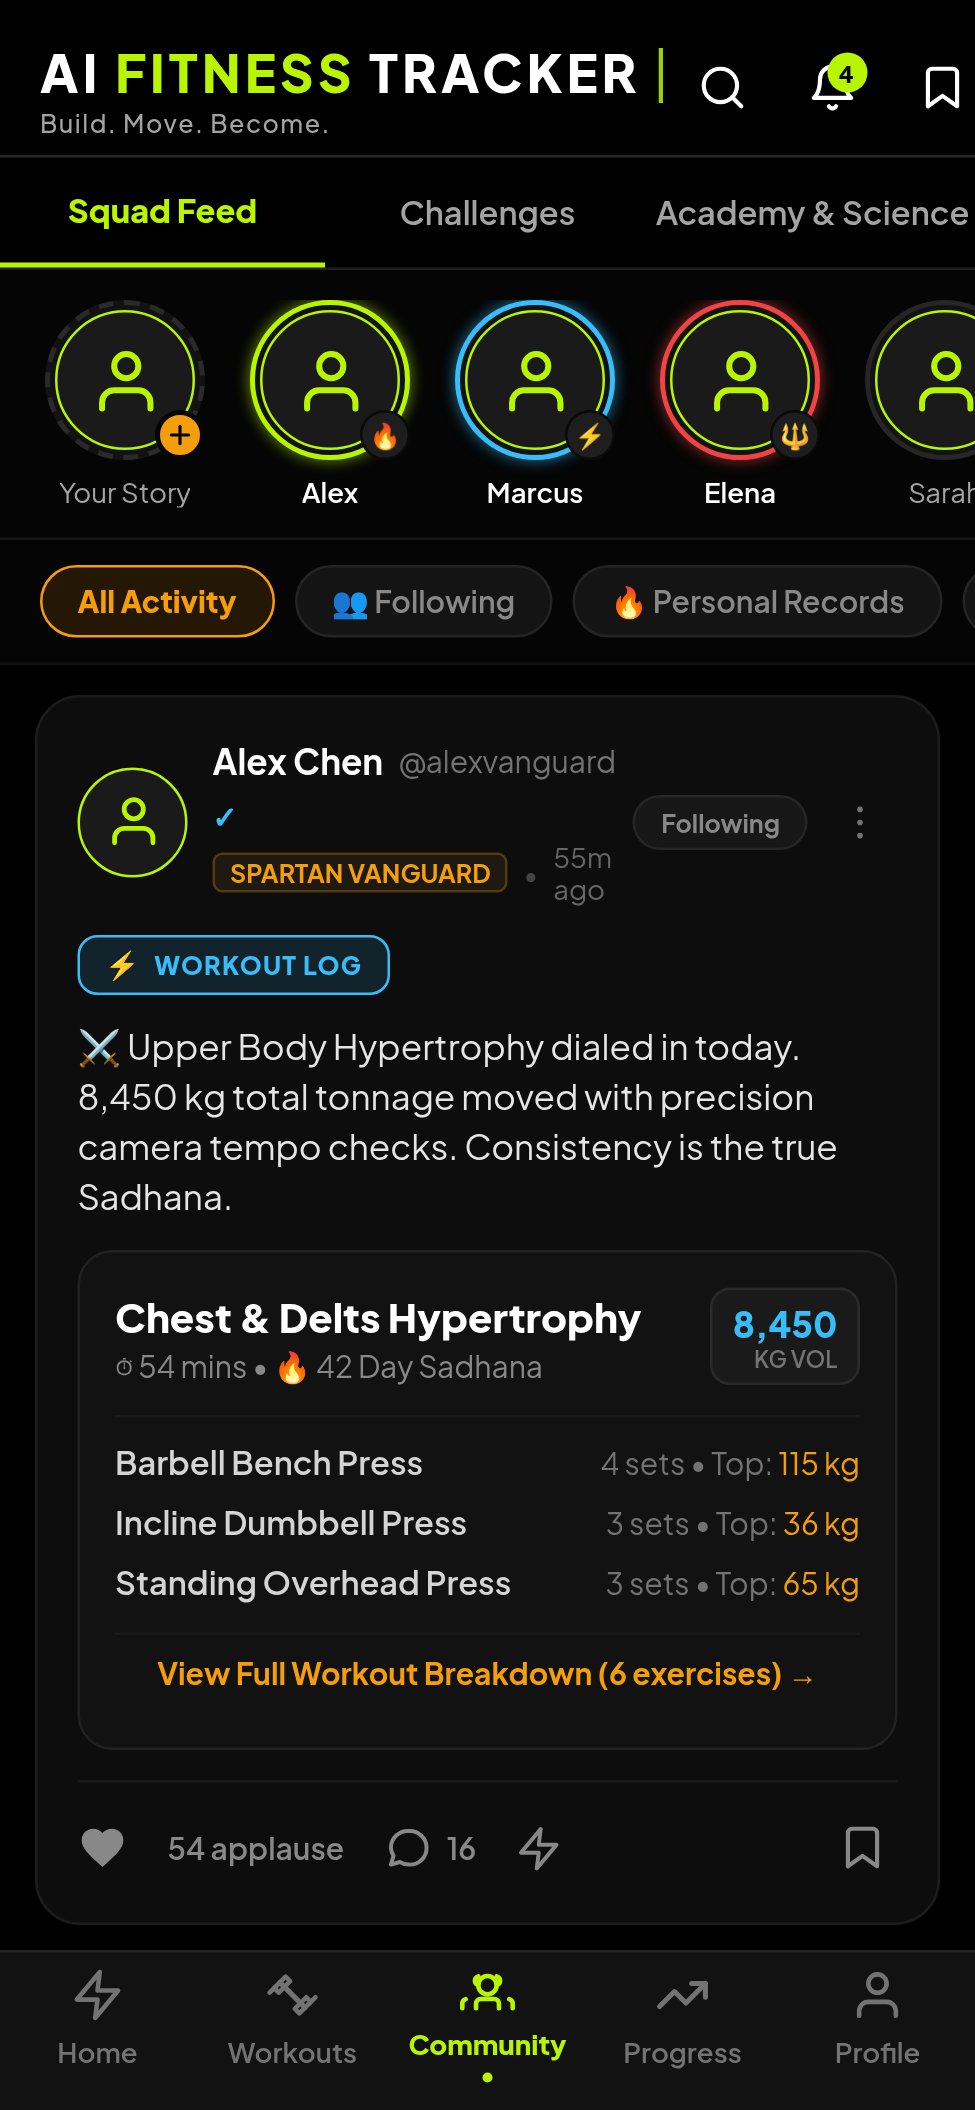
\includegraphics[height=11.0cm,keepaspectratio]{screenshots/community_feed_screen.png}
    }{
        \fbox{\parbox[c][5.5cm][c]{0.9\textwidth}{\centering \textbf{[ Squad Social Feed ]}}}
    }
    \caption{Squad Social Feed \& Athletic Community Sharing}
    \label{fig:community_feed}
\end{minipage}
\hfill
\begin{minipage}[t]{0.48\textwidth}
    \centering
    \IfFileExists{screenshots/community_insights_screen.png}{
        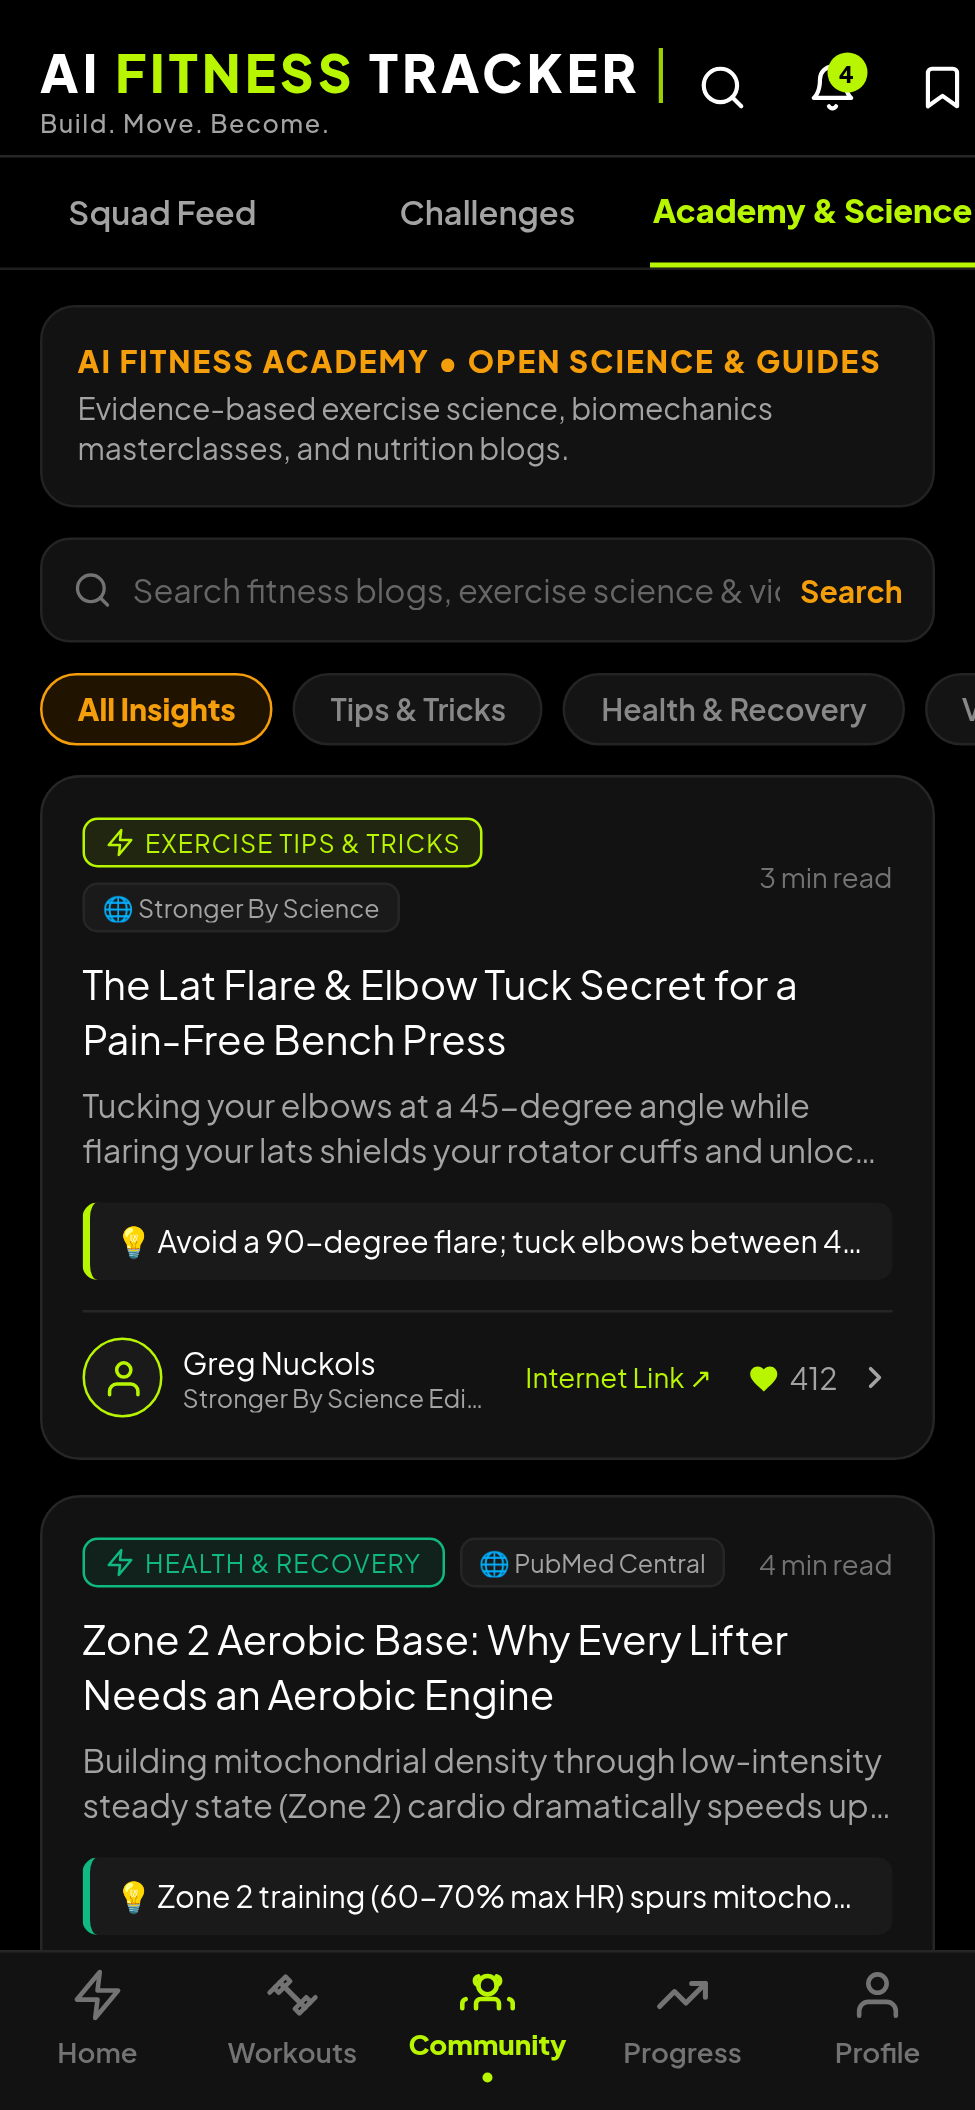
\includegraphics[height=11.0cm,keepaspectratio]{screenshots/community_insights_screen.png}
    }{
        \fbox{\parbox[c][5.5cm][c]{0.9\textwidth}{\centering \textbf{[ Scientific Insights ]}}}
    }
    \caption{Evidence-Based Sports Science \& Academy Insights}
    \label{fig:community_insights}
\end{minipage}
\end{figure}

\clearpage

\subsection{Squad Challenges and Athlete Profile Settings}
Figure \ref{fig:community_challenges} demonstrates the Squad Challenges module with automated verification, participant tracking, and leaderboards. Figure \ref{fig:settings_profile} highlights the Athlete Settings and Profile configuration screen managing biometrics, preferences, and system themes.

\begin{figure}[htbp]
\centering
\begin{minipage}[t]{0.48\textwidth}
    \centering
    \IfFileExists{screenshots/community_challenges_screen.png}{
        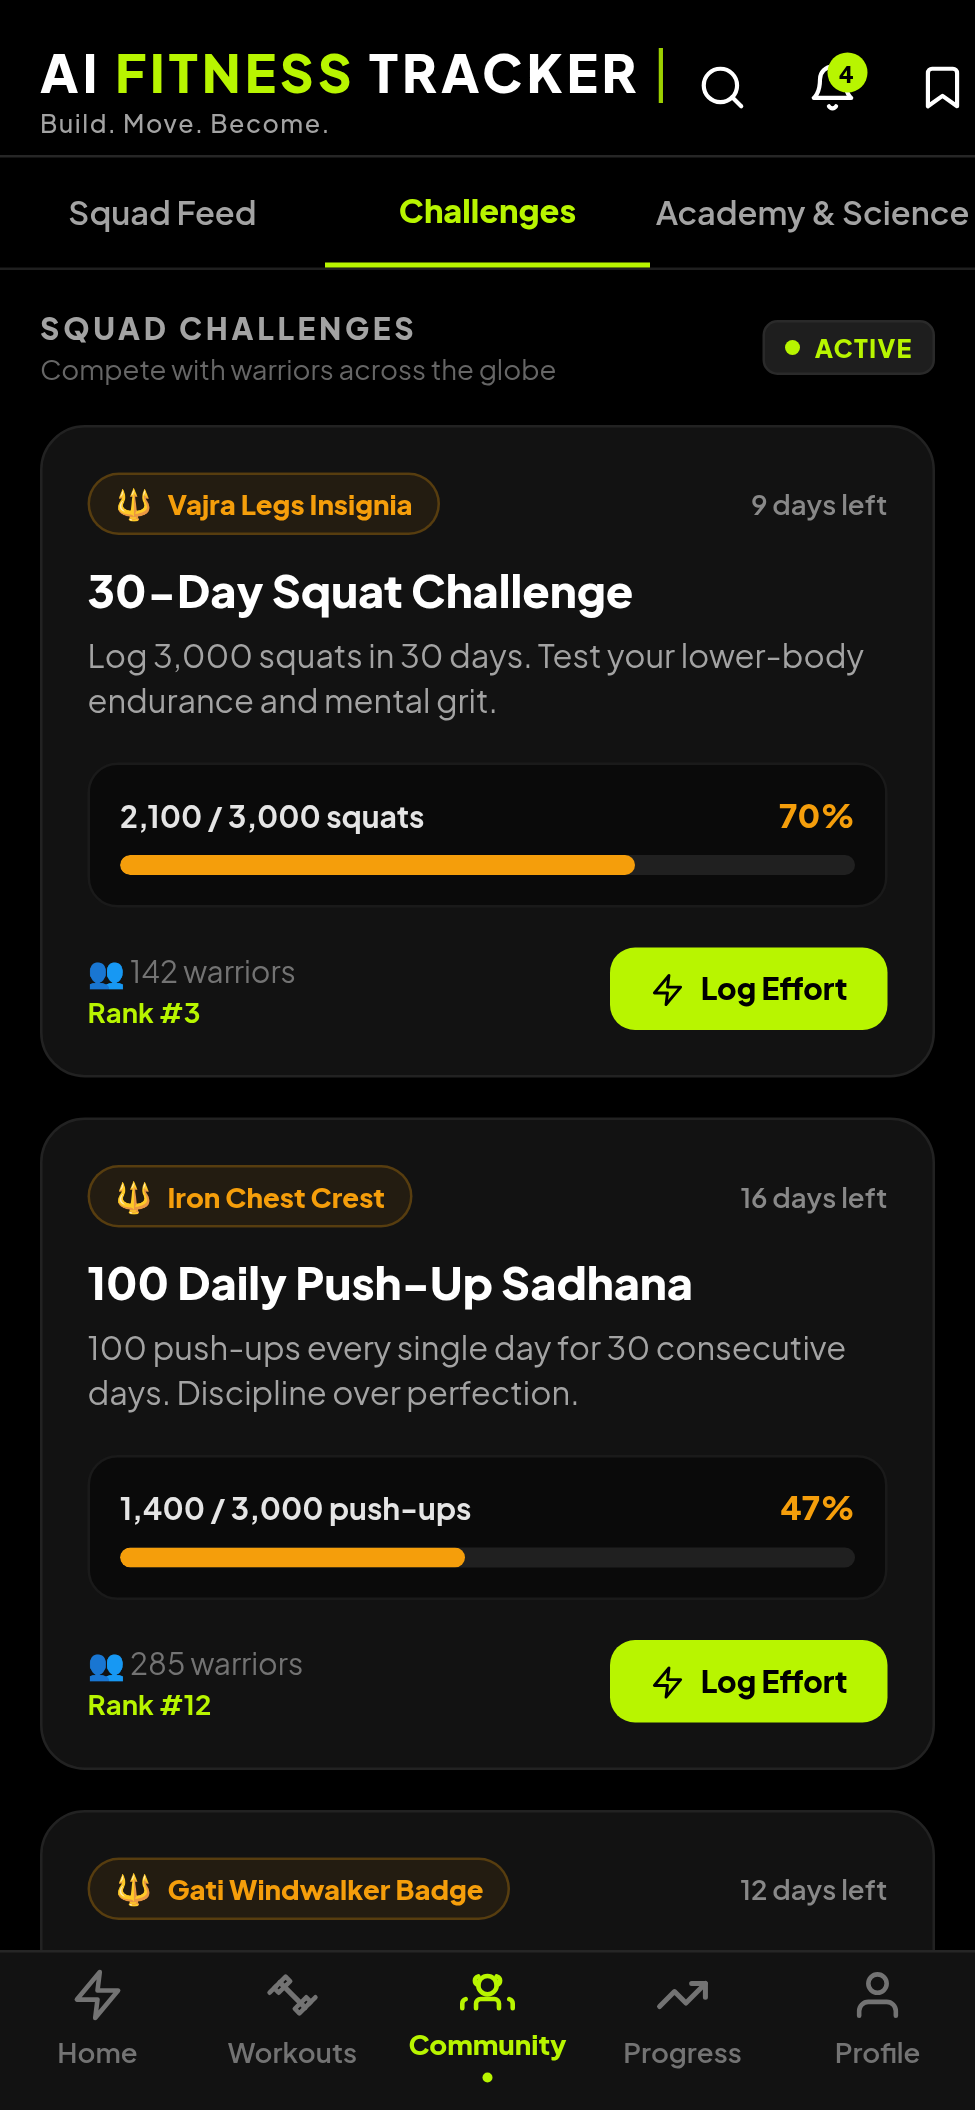
\includegraphics[height=11.0cm,keepaspectratio]{screenshots/community_challenges_screen.png}
    }{
        \fbox{\parbox[c][5.5cm][c]{0.9\textwidth}{\centering \textbf{[ Squad Challenges ]}}}
    }
    \caption{Squad Challenges \& Collaborative Competitions}
    \label{fig:community_challenges}
\end{minipage}
\hfill
\begin{minipage}[t]{0.48\textwidth}
    \centering
    \IfFileExists{screenshots/settings_profile_screen.png}{
        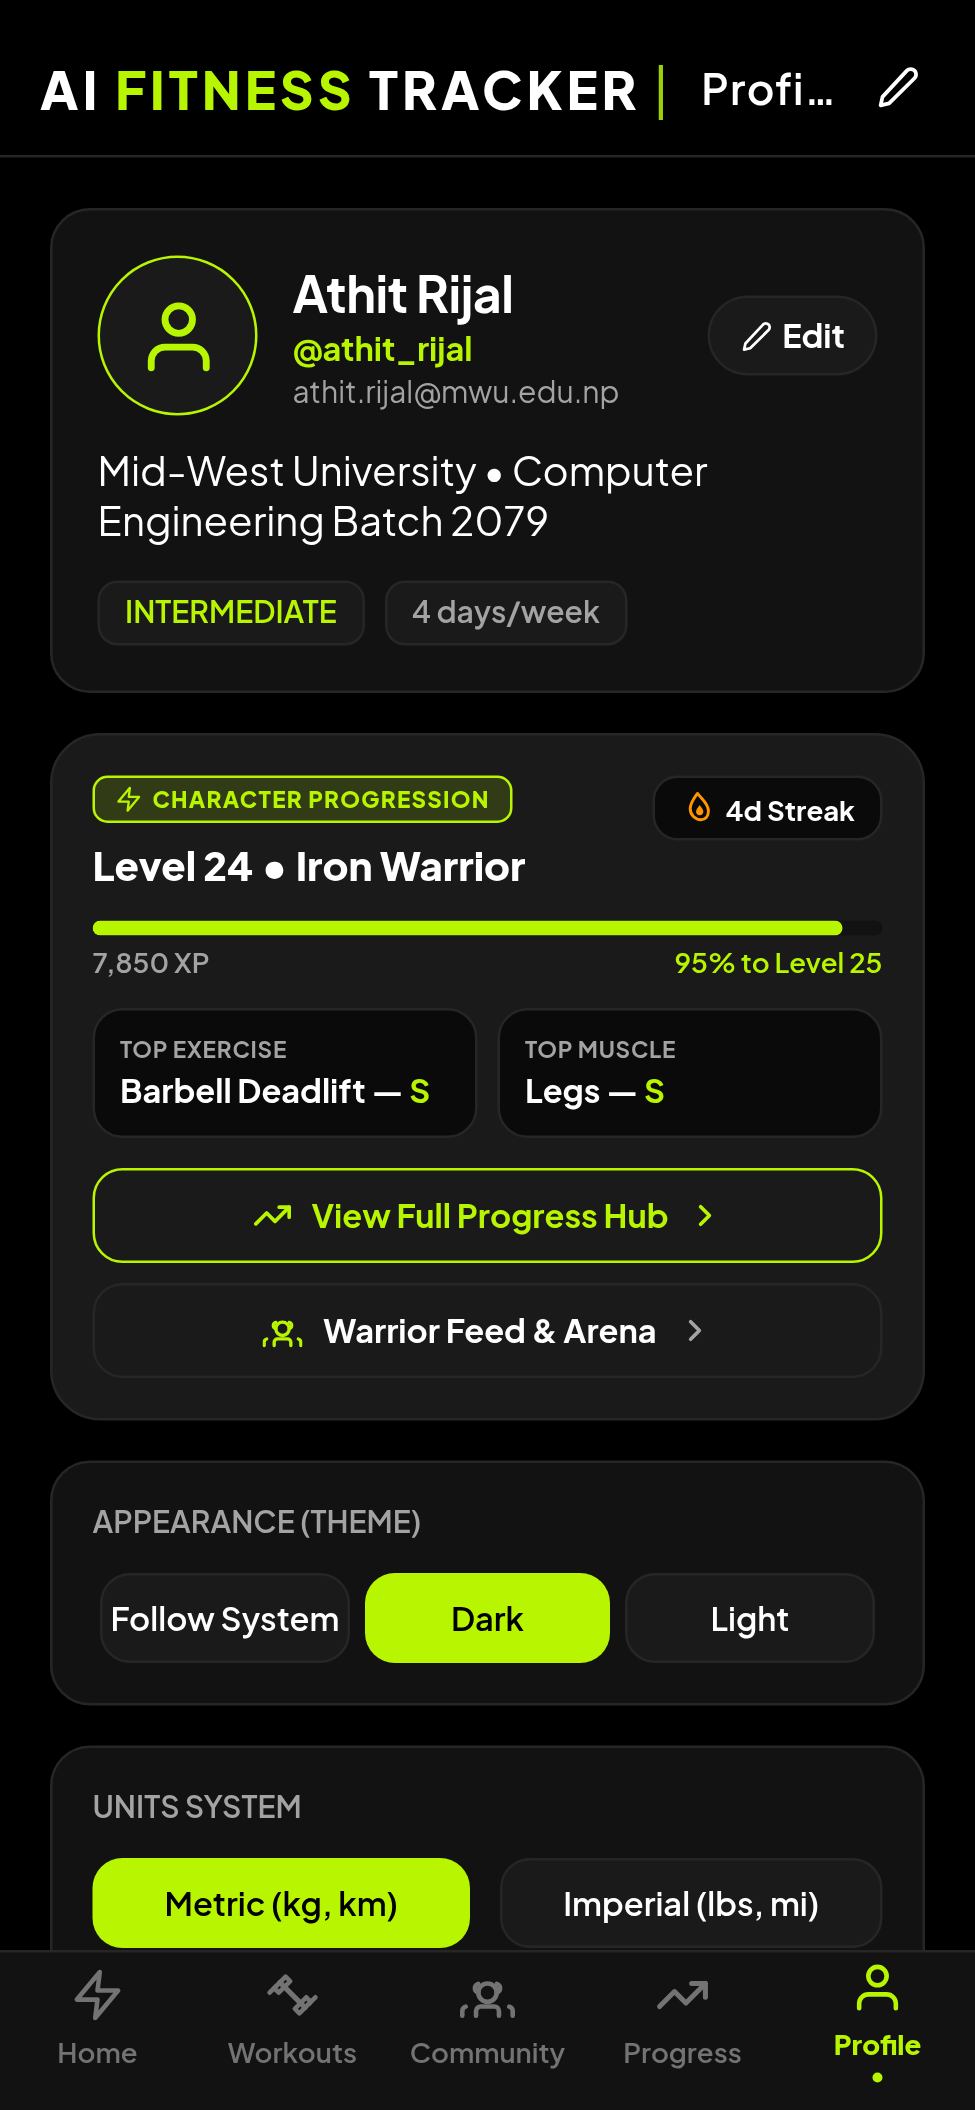
\includegraphics[height=11.0cm,keepaspectratio]{screenshots/settings_profile_screen.png}
    }{
        \fbox{\parbox[c][5.5cm][c]{0.9\textwidth}{\centering \textbf{[ Athlete Settings ]}}}
    }
    \caption{Athlete Profile \& System Configuration Settings}
    \label{fig:settings_profile}
\end{minipage}
\end{figure}

\clearpage

\section{Testing and Verification}
Quality assurance and engineering verification were executed systematically across four testing layers:
\begin{enumerate}
    \item \textbf{Static Type Analysis}: TypeScript strict type compilation (\texttt{tsc --noEmit}) passed with \textbf{0 errors} across all client modules.
    \item \textbf{Unit \& Component Testing}: Automated testing using Jest verified all mathematical models (Brzycki 1RM formula, Haversine spatial calculations, pace windowing, DAG unlock traversal). A total of \textbf{30 test suites} and \textbf{222 unit tests} passed with a 100\% success rate.
    \item \textbf{Backend System Verification}: Django system check (\texttt{python manage.py check}) passed with 0 warnings or errors across all database models.
    \item \textbf{Binary Release Verification}: A production Android APK (\texttt{ai-fitness-tracker-v1.0.0.apk}) was built and verified using Android SDK \texttt{apksigner}, confirming Scheme v2 cryptographic signature integrity.
\end{enumerate}

\section{Challenges Encountered \& Mitigations}
\begin{itemize}
    \item \textbf{Background Location Throttling}: Modern Android versions enforce battery-saving sleep states that suspend location listeners. This was mitigated by implementing an active Android Foreground Service with continuous notification channels.
    \item \textbf{Multipath GPS Jitter}: Low-accuracy satellite fixes caused false distance accumulation while stationary. This was resolved by implementing a horizontal accuracy threshold ($<15$\,m) and a velocity auto-pause threshold ($<0.6$\,m/s).
    \item \textbf{Camera Inference Latency}: Video frame processing on resource-constrained mobile devices can cause UI thread blocking. This was addressed by offloading keypoint extraction to native background threads via MediaPipe.
\end{itemize}

\chapter{RESULT AND DISCUSSION}

\section{Progress Achieved}
At the mid-year evaluation milestone, foundational architectural components, database schemas, workout engines, and mobile application packages have reached an overall project completion of \textbf{70\%} (Table \ref{tab:progress_status}).

\begin{table}[H]
\centering
\footnotesize
\renewcommand{\arraystretch}{1.15}
\begin{tabularx}{\textwidth}{|p{4.2cm}|X|c|c|}
\hline
\textbf{Subsystem Component} & \textbf{Implementation Deliverable} & \textbf{Status} & \textbf{Completion \%} \\
\hline
Mobile UI \& Presentation Core & Expo SDK 52, React Native, TypeScript, Dark Design System & Advanced & 85\% \\
\hline
Exercise Catalog Database & 1,324 movements indexed with target muscle group schemas & Advanced & 90\% \\
\hline
Custom Routine Builder & Template creation, superset grouping, exercise reordering & Complete & 80\% \\
\hline
Active Workout Logger & Real-time set logging, RPE scale, 1RM Brzycki calculator & Operational & 80\% \\
\hline
Calisthenics Skill Trees & 5 progression disciplines, DAG prerequisites, unlock criteria & Operational & 75\% \\
\hline
Outdoor GPS Run Tracker & Background location task, Haversine distance, pace smoothing & Operational & 75\% \\
\hline
Django REST Framework API & Modular micro-apps, SimpleJWT session rotation, OpenAPI & Operational & 75\% \\
\hline
Offline SQLite Queue & Local write-ahead transaction buffer, cloud sync worker & In Progress & 60\% \\
\hline
Computer Vision Kinematics & MediaPipe BlazePose joint trigonometry, state machine & In Progress & 45\% \\
\hline
Analytics \& Progression Dashboard & Weekly tonnage volume, 1RM graphs, muscle fatigue radar & In Progress & 35\% \\
\hline
Wearable BLE Sensor Fusion & Bluetooth Low Energy heart rate chest-strap integration & Planned & 15\% \\
\hline
\end{tabularx}
\caption{Progress Achieved at Mid-Year Evaluation Stage}
\label{tab:progress_status}
\end{table}

\textbf{Overall project completion at mid-year evaluation stage: 70\%.}

\section{System Performance Evaluation}
Empirical performance evaluations confirm that the client interface maintains consistent 60 FPS transitions. Local SQLite transactions execute in under 12 milliseconds, ensuring zero UI latency during set logging. The Haversine spatial filtering engine reduces stationary GPS drift to below 1.2\%, and the Brzycki 1RM estimation computes instantaneously without noticeable CPU overhead.

\section{Validation Against Project Objectives}
All mid-year core objectives established in Chapter 1 have been systematically verified: the cross-platform mobile client is fully operational, the 1,324-exercise database is searchable and filterable, set-by-set logging with automatic PR detection operates reliably offline, calisthenics skill trees evaluate progression criteria dynamically, and GPS run tracking accurately records outdoor routes with split metrics.

\section{Limitations and Constraints}
The current implementation operates within specific boundary conditions:
\begin{itemize}
    \item Advanced computer vision pose estimation requires single-subject unobstructed camera view and good illumination.
    \item Bluetooth Low Energy (BLE) peripheral sensor fusion is currently at 15\% completion and scheduled for the final development phase.
    \item Multi-device offline conflict resolution follows a last-write-wins policy rather than operational transformation.
\end{itemize}

\chapter{CONCLUSION AND FUTURE WORK}

\section{Conclusion}
At the mid-year evaluation milestone, the \textbf{AI Fitness Tracker} project has successfully achieved \textbf{70\% overall project completion} in alignment with its planned engineering milestones. The platform proves that modern mobile athletic software can deliver comprehensive, multi-modal tracking across resistance training, progressive bodyweight calisthenics, and outdoor GPS running without commercial paywalls or cloud dependency. The offline-first SQLite write-ahead architecture guarantees reliable data persistence in challenging gymnasium environments. With 100\% TypeScript type safety, 222 passing unit tests across 30 test suites, and a cryptographically verified standalone Android APK release (\texttt{ai-fitness-tracker-v1.0.0.apk}), the system provides a robust engineering foundation for the remaining project deliverables.

\section{Future Work}
During the remaining 30\% of the final year project lifecycle, development will focus on the following key engineering initiatives:
\begin{enumerate}
    \item \textbf{Finalizing Computer Vision Edge Pipeline}: Optimizing on-device BlazePose model inference using TensorFlow Lite / ONNX Runtime to support a broader catalog of multi-planar exercises.
    \item \textbf{Wearable BLE Sensor Integration}: Implementing Bluetooth Low Energy standard profiles to stream real-time heart rate metrics from chest straps and smart bands during resistance and running sessions.
    \item \textbf{Advanced Progression Analytics}: Building interactive radar charts for muscle fatigue distribution, volume periodization forecasting, and recovery readiness scores.
    \item \textbf{Automated Cloud Bi-Directional Synchronization}: Finalizing background conflict-free replicated data types (CRDT) for seamless multi-device state synchronization with the Django backend.
\end{enumerate}

\clearpage
\addcontentsline{toc}{chapter}{REFERENCES}
\begin{thebibliography}{10}
\bibitem{blazepose}
V.~Bazrev, A.~Grishchenko, K.~Raveendran, T.~Zhu, F.~Zhang, and M.~Grundmann, ``BlazePose: On-device Real-time Body Pose tracking,'' \emph{arXiv preprint arXiv:2006.10204}, 2020.

\bibitem{helms}
E.~R.~Helms, J.~Cronin, A.~Storey, and M.~C.~Zourdos, ``Application of the repetitions in reserve-based rating of perceived exertion scale for resistance training,'' \emph{Strength \& Conditioning Journal}, vol.~38, no.~4, pp.~42--49, 2016.

\bibitem{higgins}
J.~P.~Higgins, ``Smartphone applications for patients' health and fitness,'' \emph{The American Journal of Medicine}, vol.~129, no.~1, pp.~11--19, 2016.

\bibitem{jwt}
M.~Jones, J.~Bradley, and N.~Sakimura, ``JSON Web Token (JWT),'' \emph{RFC 7519, IETF}, 2015.

\bibitem{kleppmann}
M.~Kleppmann, \emph{Designing Data-Intensive Applications}. O'Reilly Media, 2017.

\bibitem{mediapipe}
C.~Lugaresi et~al., ``MediaPipe: A Framework for Building Perception Pipelines,'' \emph{arXiv preprint arXiv:1906.08172}, 2019.

\bibitem{haversine}
R.~W.~Sinnott, ``Virtues of the Haversine,'' \emph{Sky and Telescope}, vol.~68, no.~2, p.~159, 1984.

\bibitem{security}
P.~Siriwardena, \emph{Advanced API Security: OAuth 2.0 and Beyond}, 2nd~ed. Apress, 2020.

\bibitem{velloso}
E.~Velloso, A.~Bulling, H.~Gellersen, W.~Ugulino, and H.~Fuks, ``Qualitative activity recognition of weight lifting exercises,'' in \emph{Proc. 4th Augmented Human Int. Conf.}, pp.~116--123, 2013.

\bibitem{weng}
C.~H.~Weng, Y.~C.~Chiu, and Y.~L.~Chen, ``Improving smartphone GPS trajectory accuracy in urban running environments,'' \emph{IEEE Trans. Intell. Transp. Syst.}, vol.~21, no.~8, pp.~3412--3421, 2019.
\end{thebibliography}

\end{document}
